
\subsection{Method}
We use a version of Kneser-Ney Smoothing.
For a sequence $w_1\dots w_k$, let $N(w_{1\dots k})$ be the number of times $w_{1\dots k}$ occurs in the training set.
The unigram probabilities are estimated as
\begin{equation}
	p_1(w_t) :=   \frac{N(w_t) + \delta}{|Train| + |V| \cdot \delta}
\end{equation}
where $\delta \in \mathbb{R}_+$ is a hyperparameter.
Here $|Train|$ is the number of tokens in the training set, $|V|$ is the number of types occurring in train or held-out data.
Higher-order probabilities $p_t(w_t|w_{0 \dots t-1})$ are estimated recursively as follows.
Let $\gamma > 0$ be a hyperparameter.
If $N(w_{0 \dots t-1}) < \gamma$, set
\begin{equation}
	p_t(w_t|w_{0 \dots t-1}) := p_{t-1}(w_t|w_{1\dots t-1})
\end{equation}
Otherwise, we interpolate between $t$-th order and lower-order estimates:
\begin{equation}
	p_t(w_t|w_{0 \dots t-1}) :=  \frac{\operatorname{max}(N(w_{0\dots t}) - \alpha, 0.0) + \alpha \cdot \#\{w : N(w_{0 \dots t-1}w) > 0\} \cdot p_{t-1}(w_t|w_{1\dots t-1})}{N(w_{0\dots t-1})}
\end{equation}
where $\alpha \in [0,1]$ is also a hyperparameter.
(CITE) show that this definition results in a well-defined probability distribution, i.e., $\sum_{w \in V} p_t(w|w_{0 \dots t-1}) = 1$.

%Note that this definition guarantees $\sum_{w \in V} p_t(w|w_{0 \dots t-1}) = 1$, because
%
%$\sum_{w \in V} \operatorname{max}(N(w_{0\dots t-1}w) - \alpha, 0.0) + \alpha \cdot \#\{w' : N(w_{0 \dots t-1}w') > 0\} \cdot p_{t-1}(w|w_{1\dots t-1})$
%
%$\sum_{w \in V : N(w_{0\dots t-1} w) > 0} (N(w_{0\dots t}) - \alpha) + \alpha \cdot \sum_{w \in V} \#\{w' : N(w_{0 \dots t-1}w') > 0\} \cdot p_{t-1}(w|w_{1\dots t-1})$
%
%$\sum_{w \in V : N(w_{0\dots t-1} w) > 0} (N(w_{0\dots t}) - \alpha) + \alpha \cdot \#\{w' : N(w_{0 \dots t-1}w') > 0\}$
%
%$\sum_{w \in V} : N(w_{0\dots t-1} w) = N(w_{0\dots t-1})$


Hyperparameters $\alpha, \gamma, \delta$ are tuned with the same strategy as for the neural network models.


\subsection{Results}



\begin{center}
\begin{longtable}{ccccccccccccccclll}
Afrikaans & Amharic & Arabic & Armenian
 \\ 
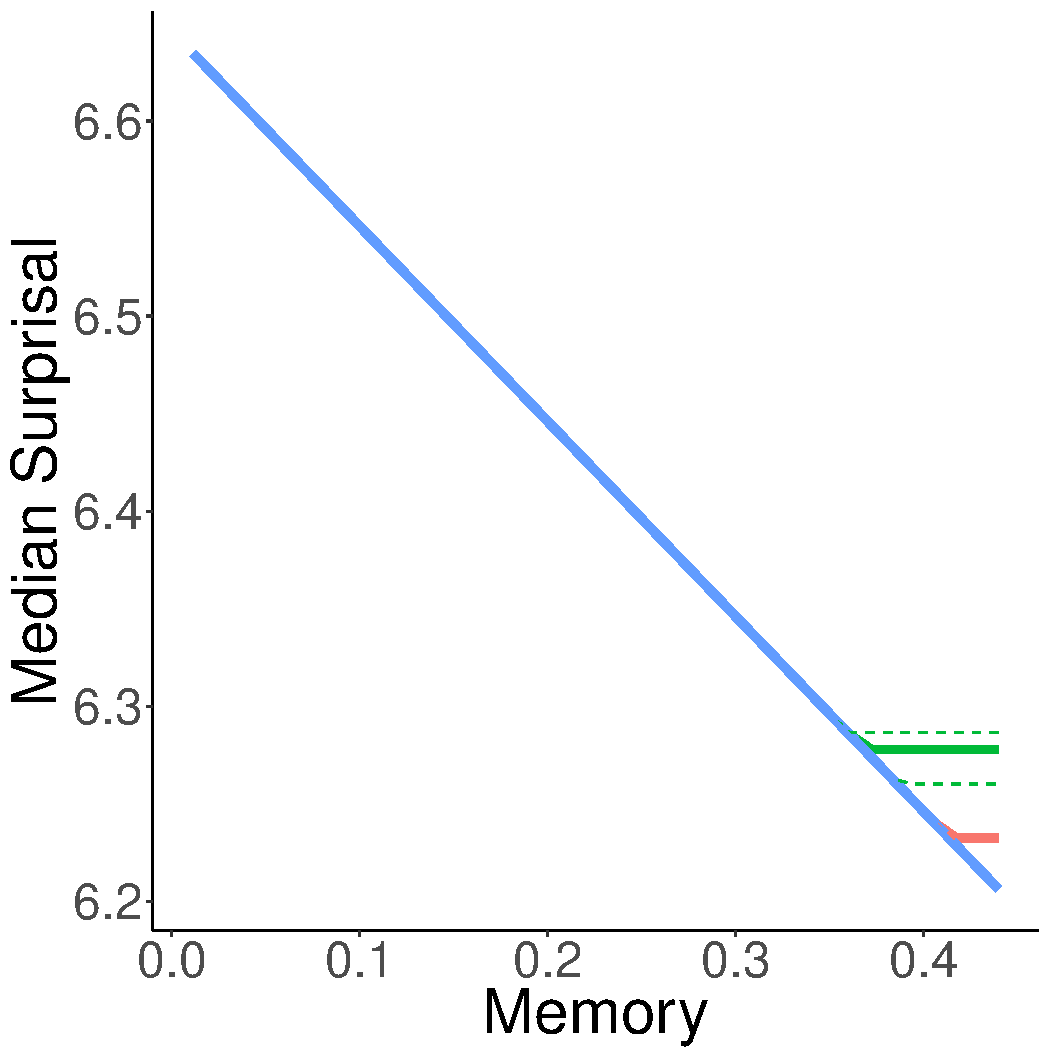
\includegraphics[width=0.25\textwidth]{../code/analyze_ngrams/visualize/figures/Afrikaans-listener-surprisal-memory-MEDIANS_onlyWordForms_boundedVocab.pdf} & 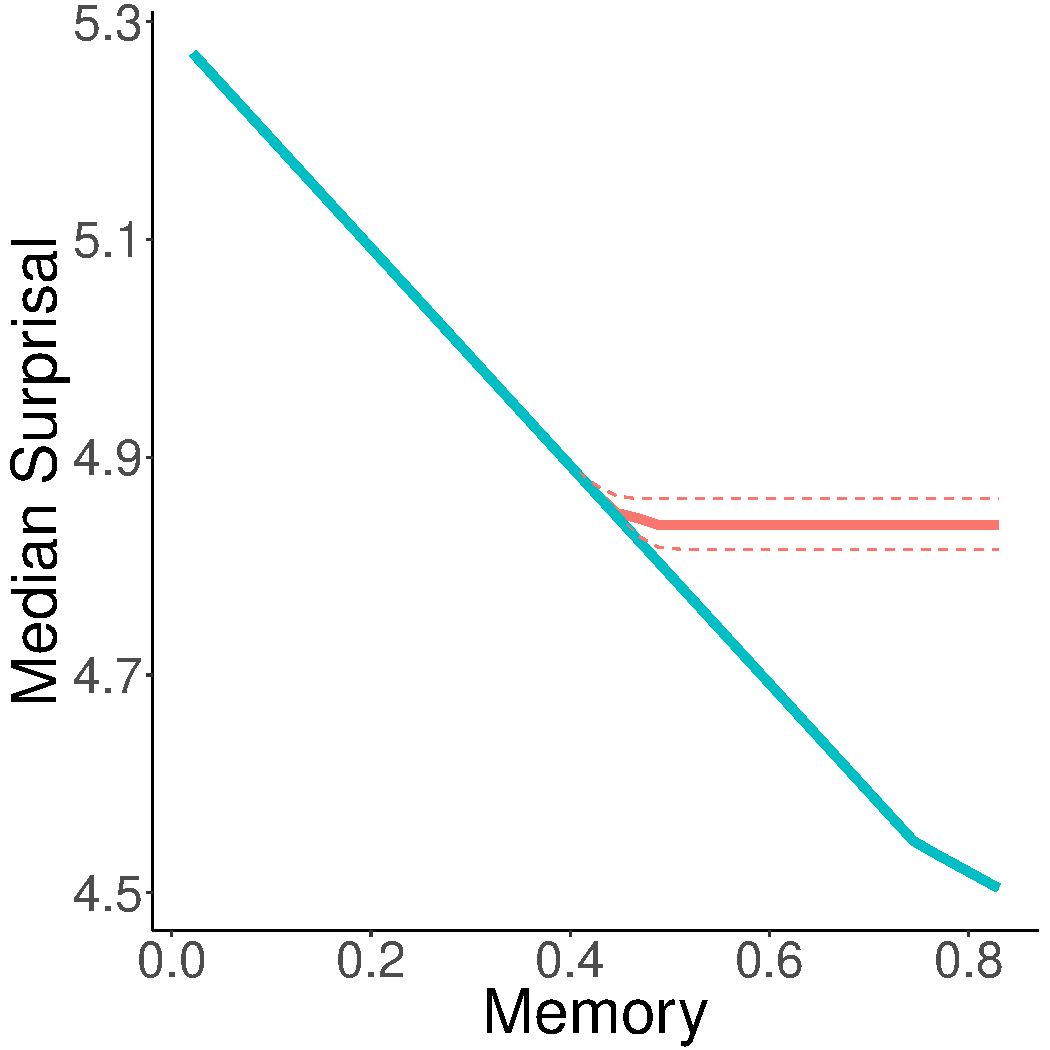
\includegraphics[width=0.25\textwidth]{../code/analyze_ngrams/visualize/figures/Amharic-Adap-listener-surprisal-memory-MEDIANS_onlyWordForms_boundedVocab.pdf} & 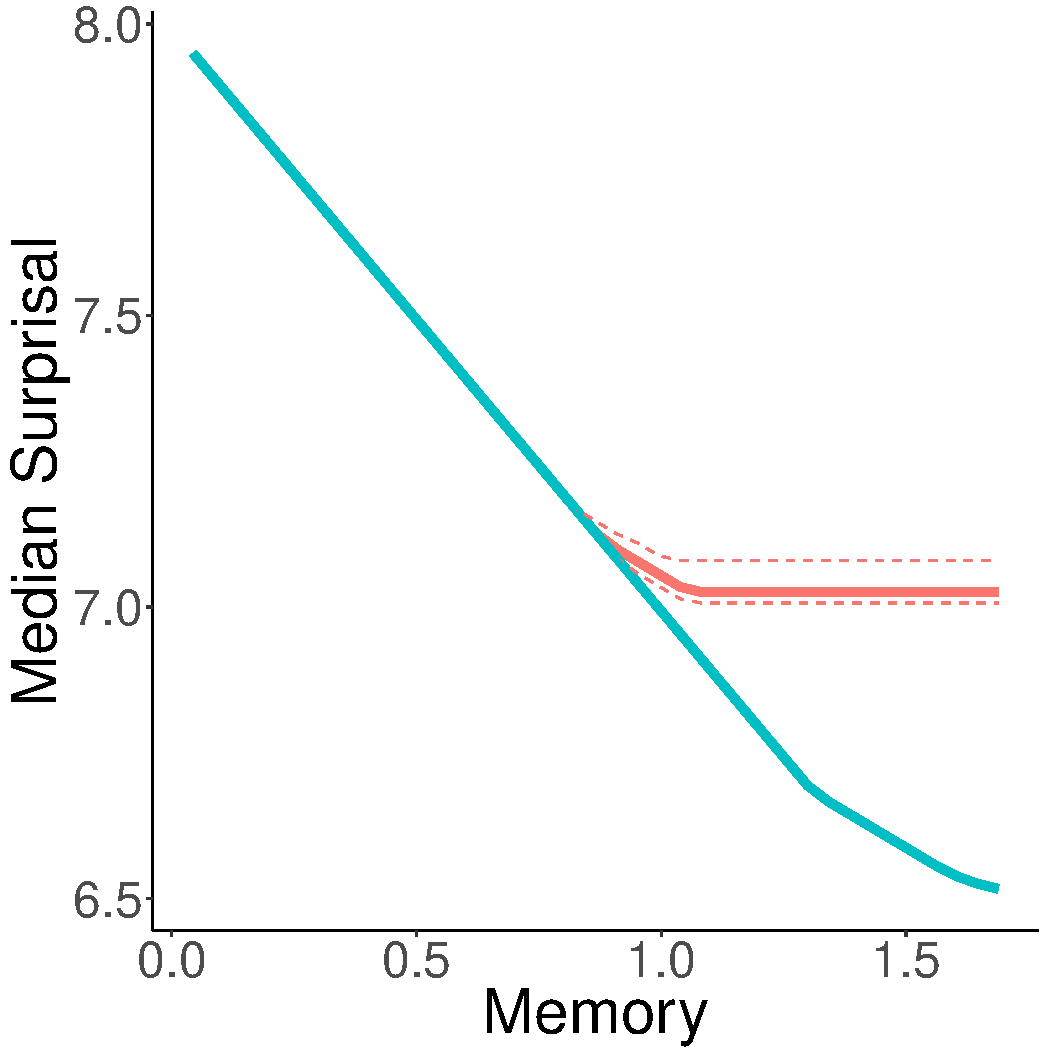
\includegraphics[width=0.25\textwidth]{../code/analyze_ngrams/visualize/figures/Arabic-listener-surprisal-memory-MEDIANS_onlyWordForms_boundedVocab.pdf} & 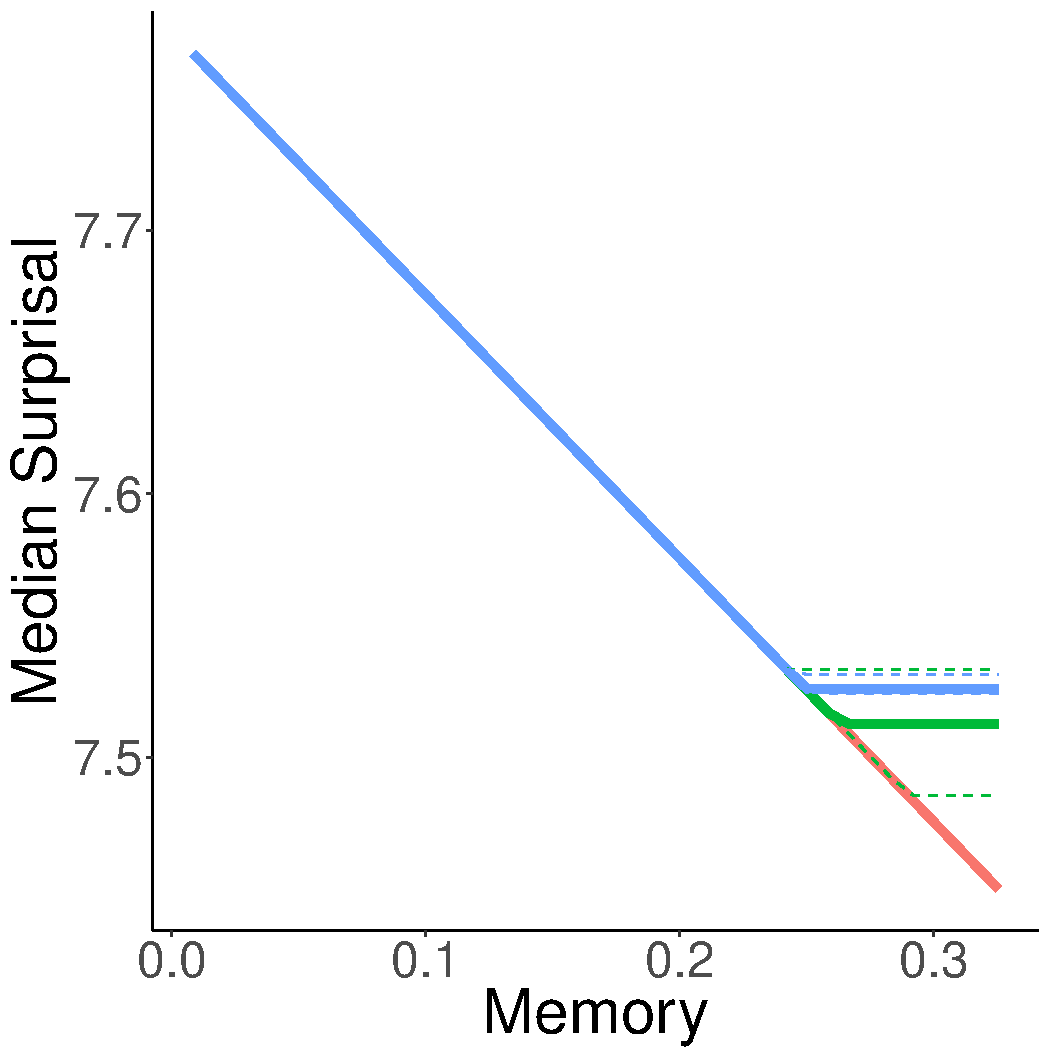
\includegraphics[width=0.25\textwidth]{../code/analyze_ngrams/visualize/figures/Armenian-Adap-listener-surprisal-memory-MEDIANS_onlyWordForms_boundedVocab.pdf}
 \\ 
Bambara & Basque & Breton & Bulgarian
 \\ 
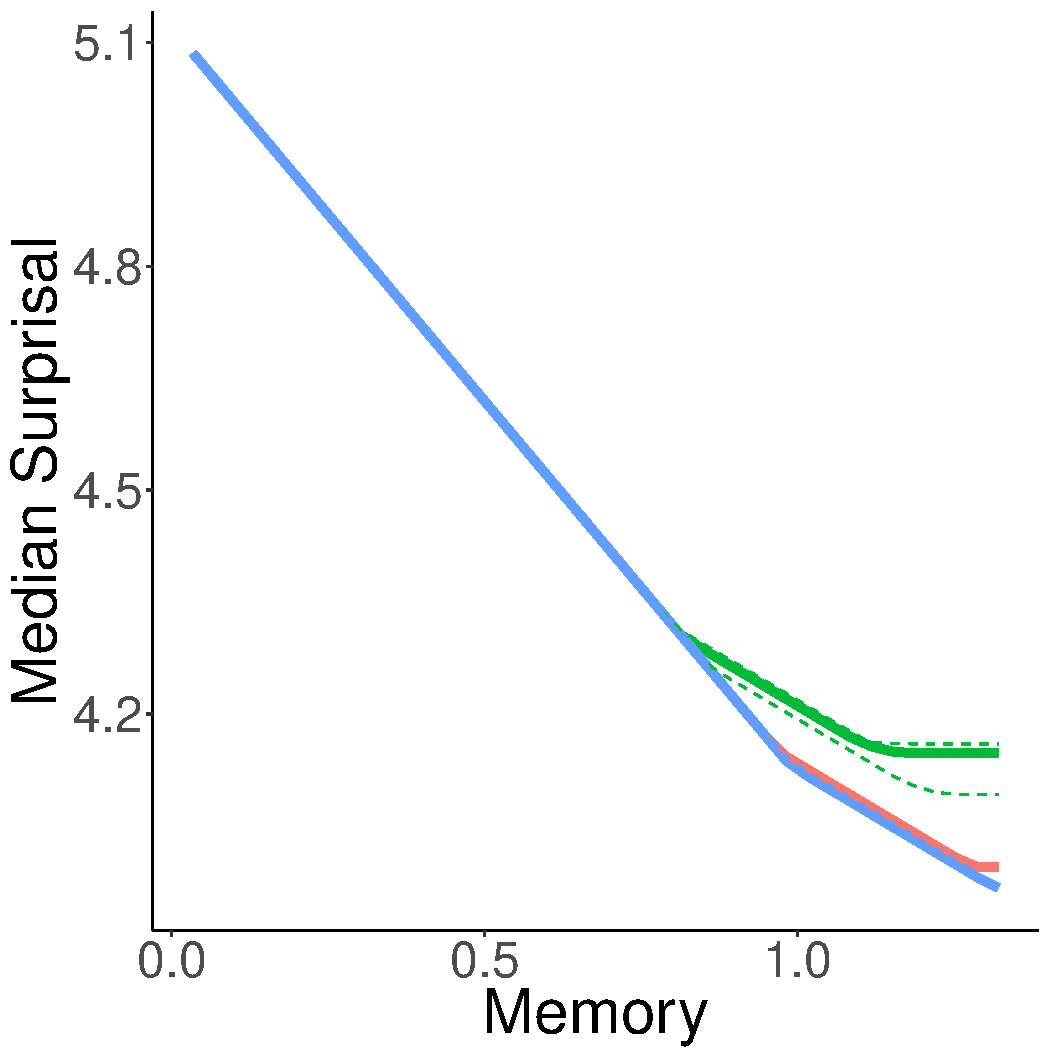
\includegraphics[width=0.25\textwidth]{../code/analyze_ngrams/visualize/figures/Bambara-Adap-listener-surprisal-memory-MEDIANS_onlyWordForms_boundedVocab.pdf} & 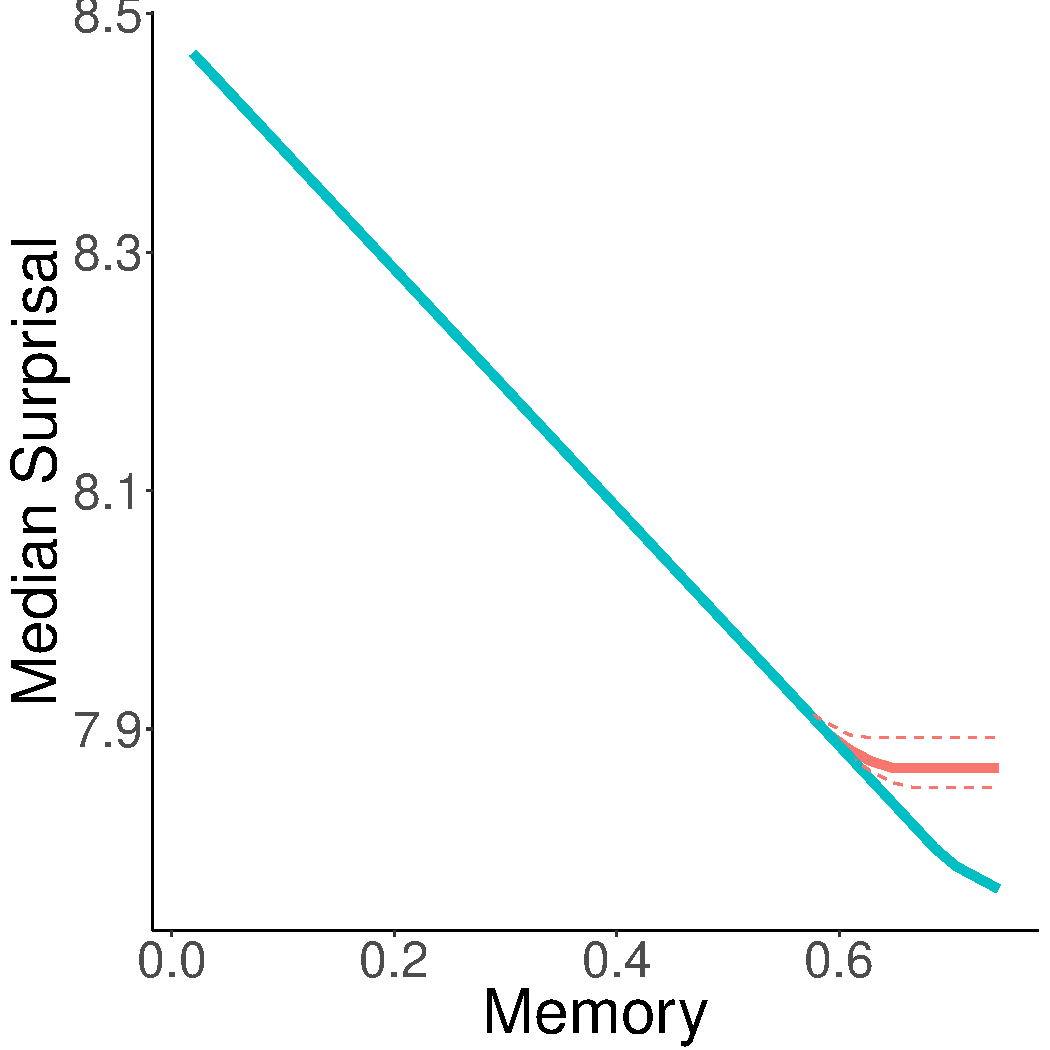
\includegraphics[width=0.25\textwidth]{../code/analyze_ngrams/visualize/figures/Basque-listener-surprisal-memory-MEDIANS_onlyWordForms_boundedVocab.pdf} & 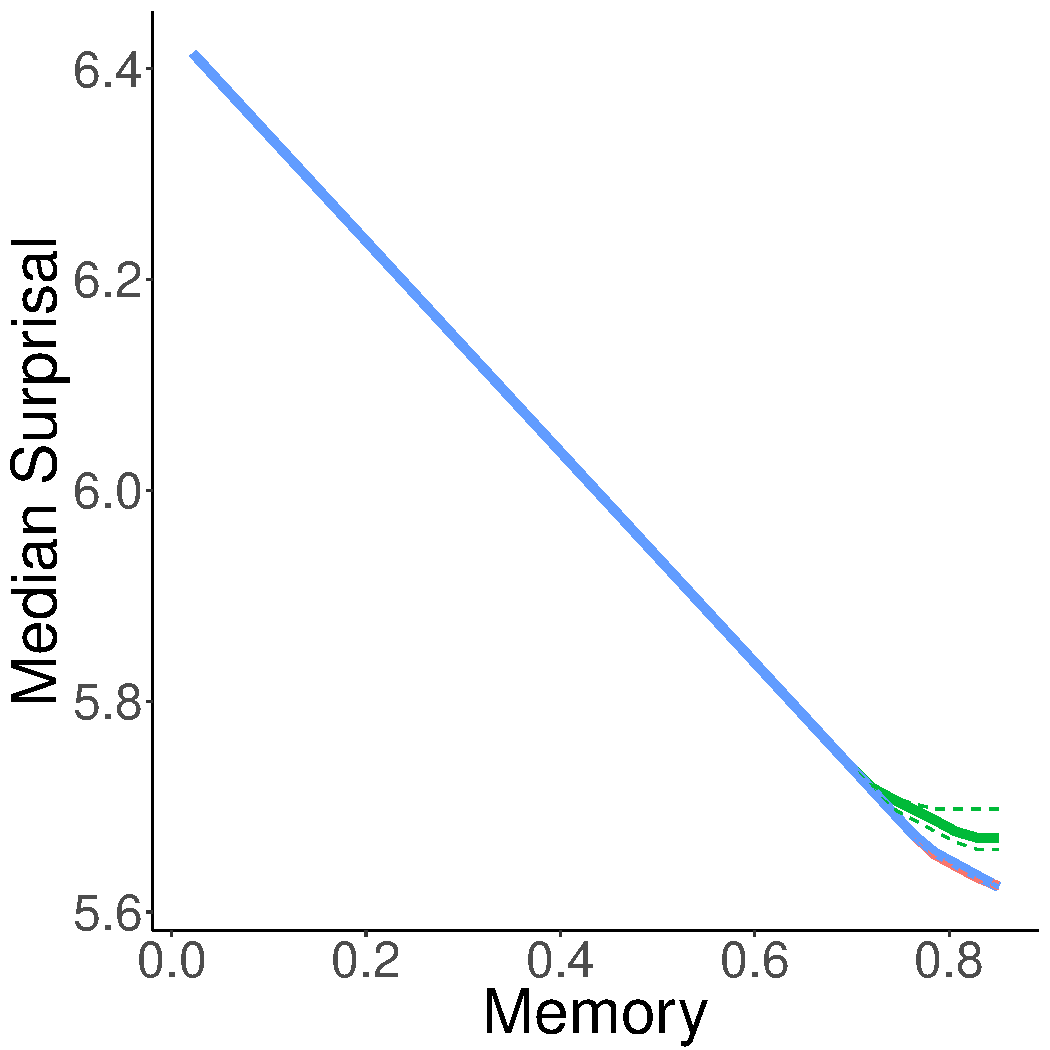
\includegraphics[width=0.25\textwidth]{../code/analyze_ngrams/visualize/figures/Breton-Adap-listener-surprisal-memory-MEDIANS_onlyWordForms_boundedVocab.pdf} & 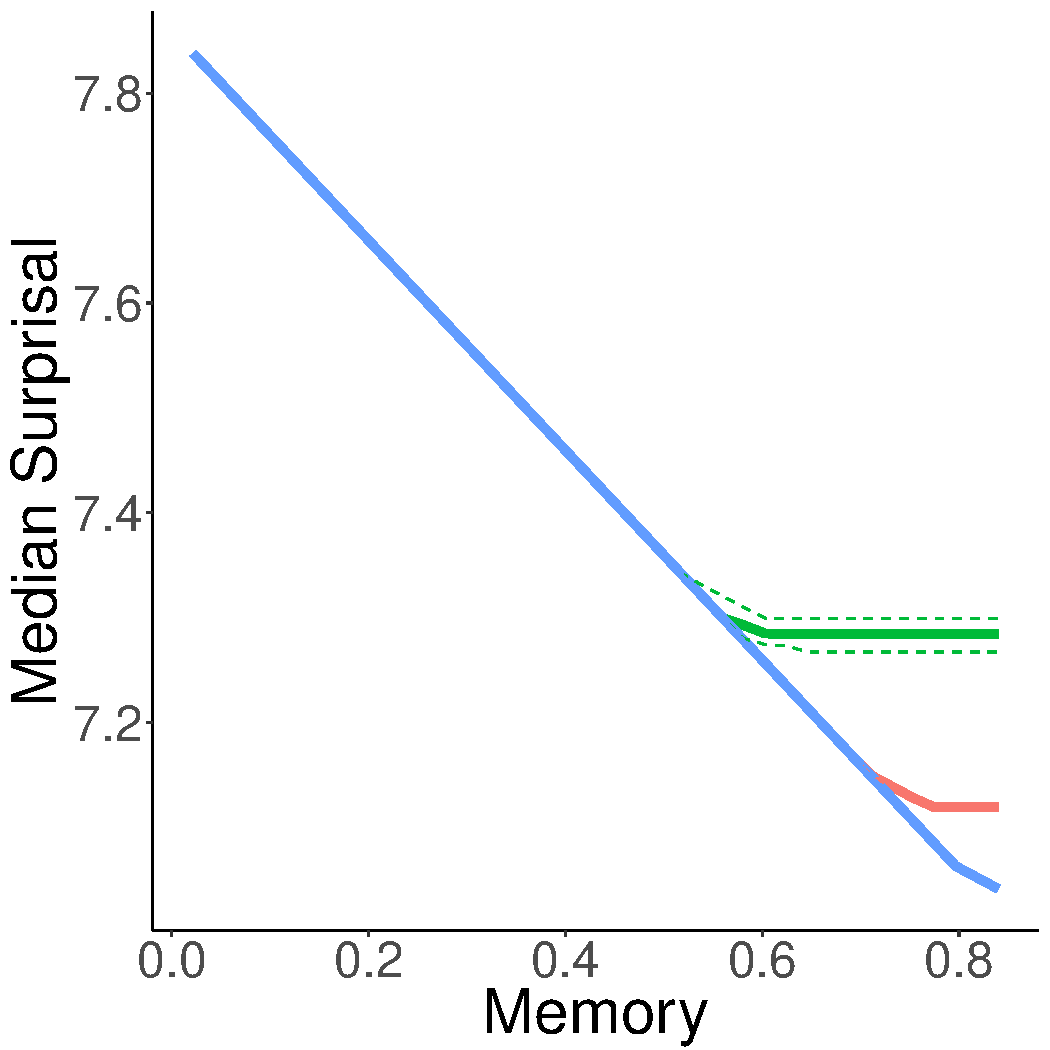
\includegraphics[width=0.25\textwidth]{../code/analyze_ngrams/visualize/figures/Bulgarian-listener-surprisal-memory-MEDIANS_onlyWordForms_boundedVocab.pdf}
 \\ 
Buryat & Cantonese & Catalan & Chinese
 \\ 
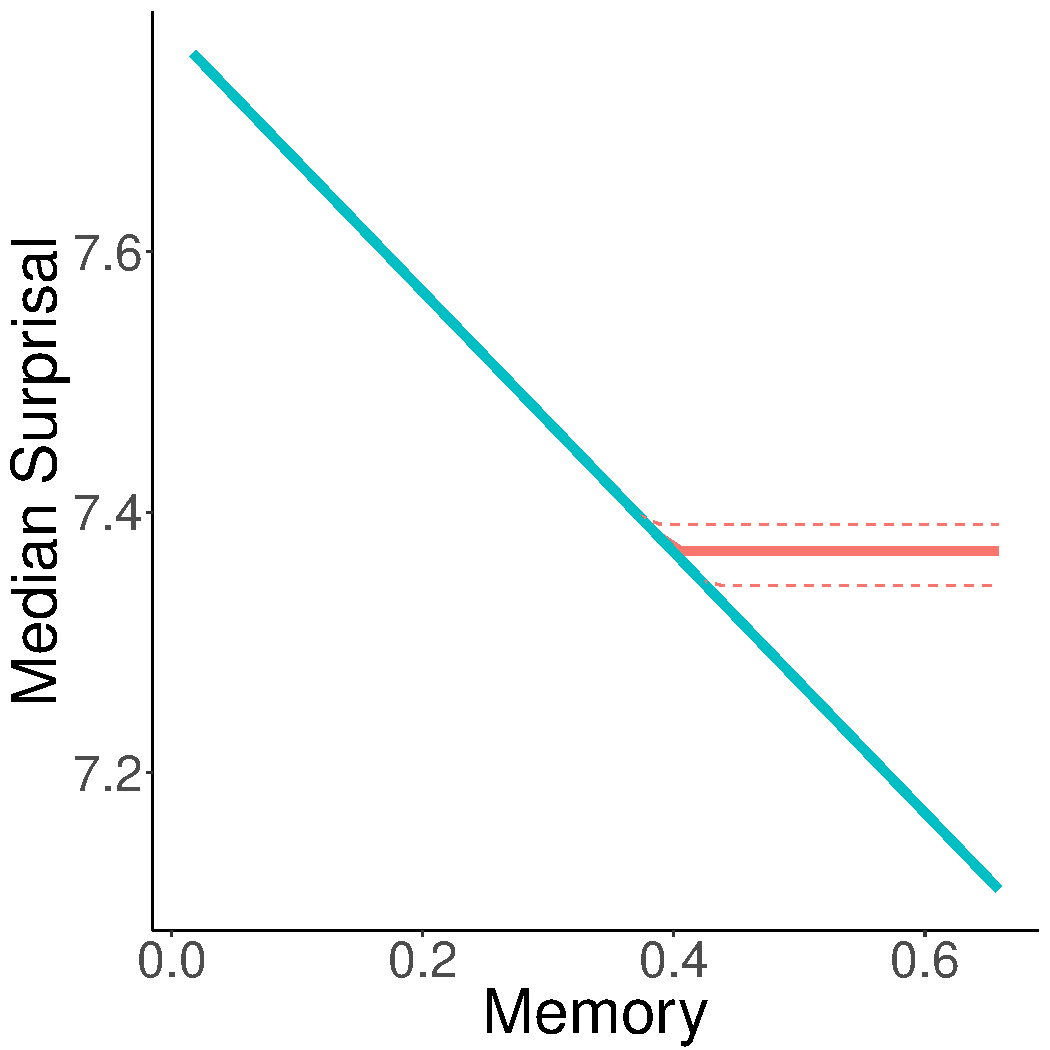
\includegraphics[width=0.25\textwidth]{../code/analyze_ngrams/visualize/figures/Buryat-Adap-listener-surprisal-memory-MEDIANS_onlyWordForms_boundedVocab.pdf} & 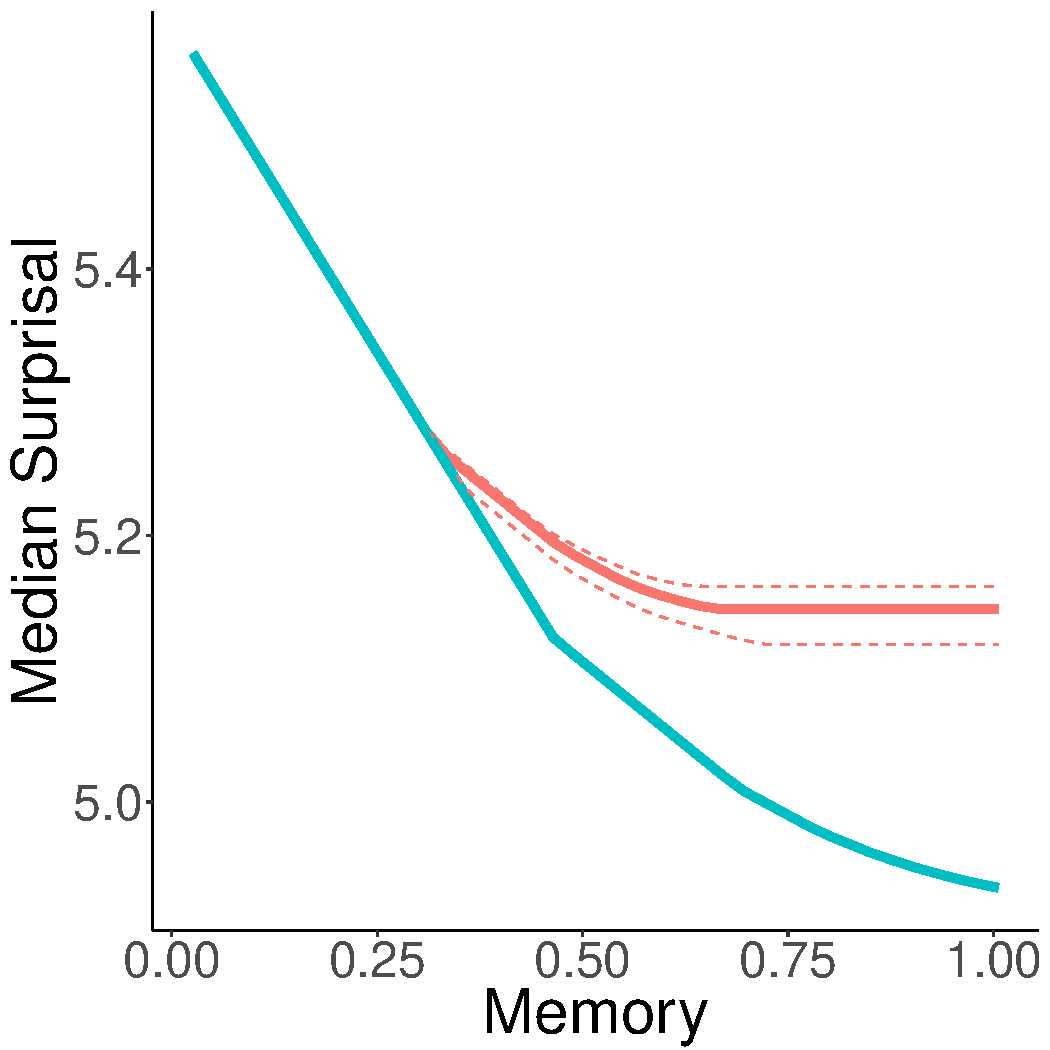
\includegraphics[width=0.25\textwidth]{../code/analyze_ngrams/visualize/figures/Cantonese-Adap-listener-surprisal-memory-MEDIANS_onlyWordForms_boundedVocab.pdf} & 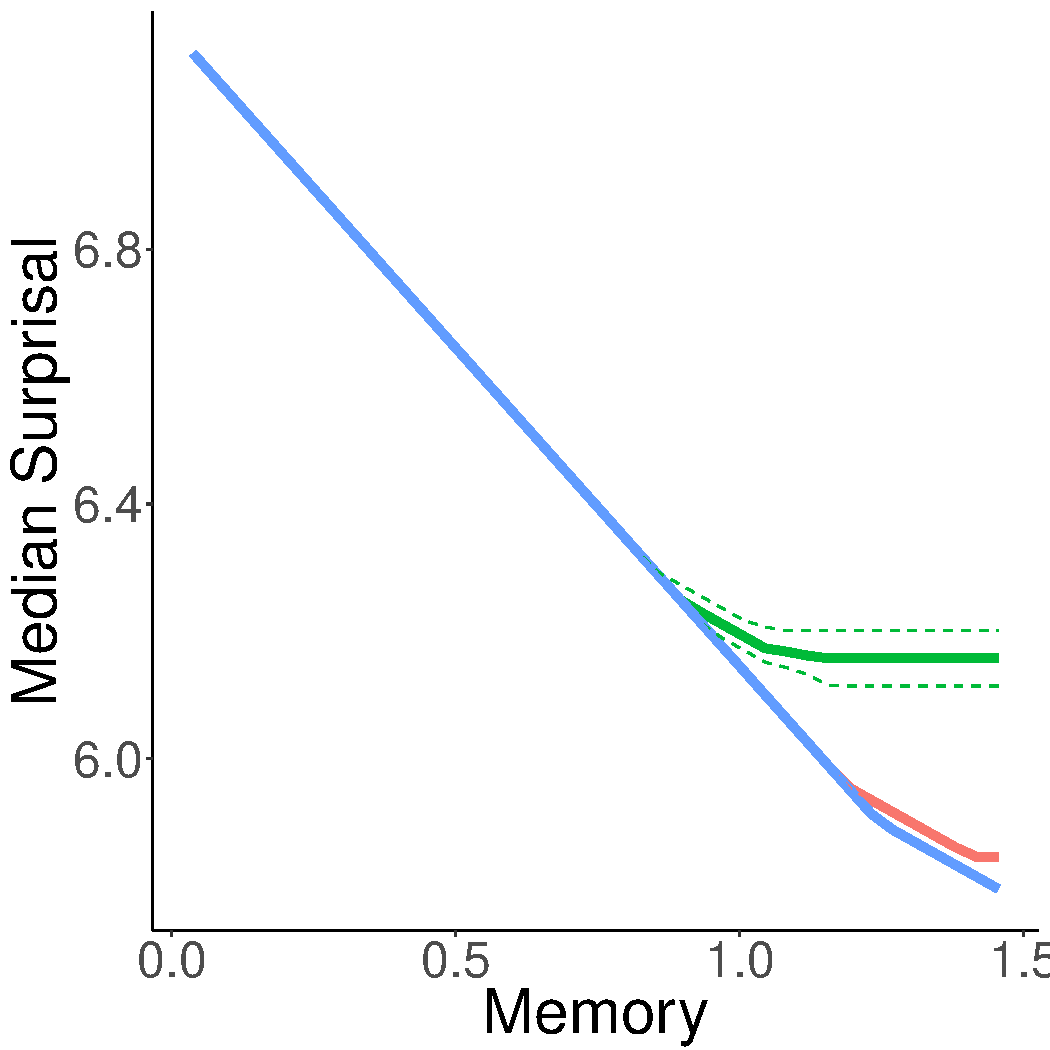
\includegraphics[width=0.25\textwidth]{../code/analyze_ngrams/visualize/figures/Catalan-listener-surprisal-memory-MEDIANS_onlyWordForms_boundedVocab.pdf} & 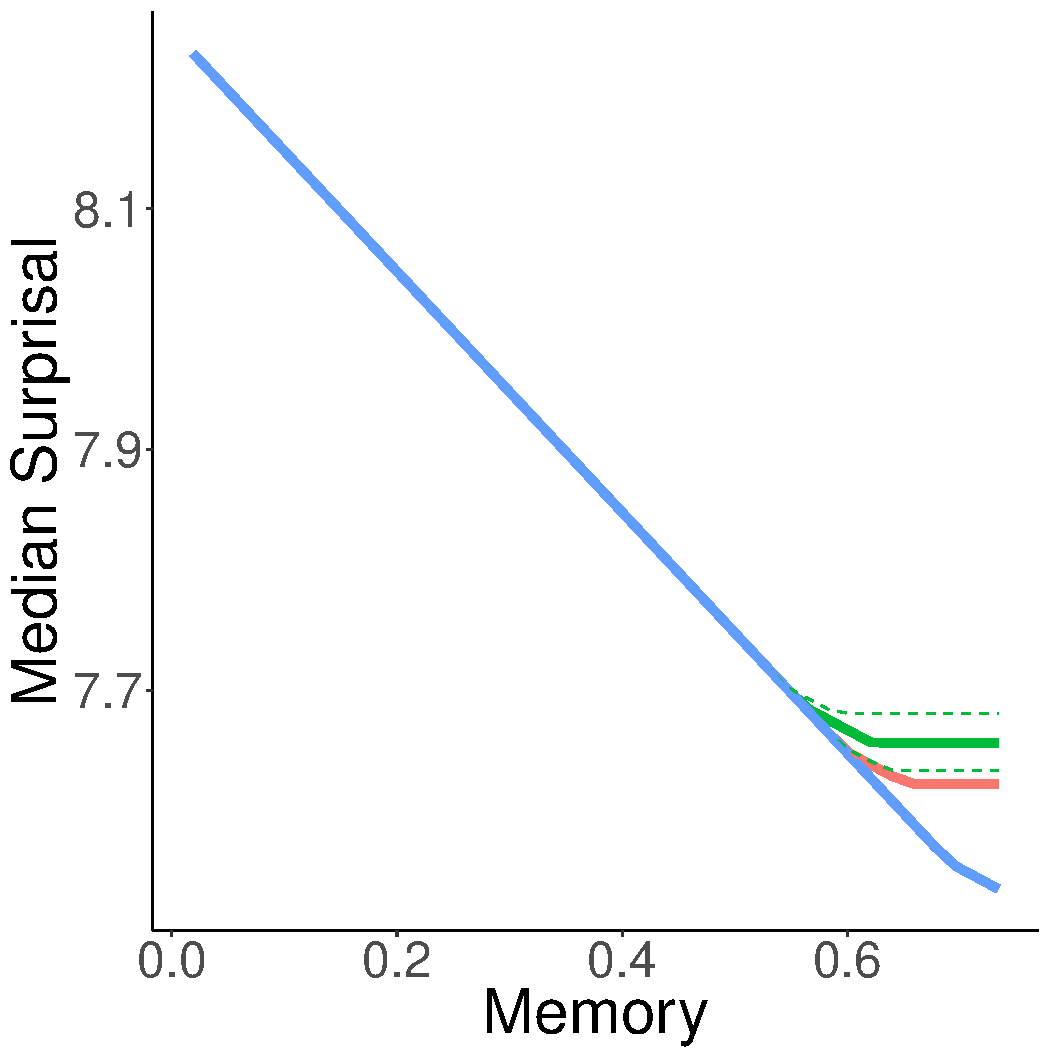
\includegraphics[width=0.25\textwidth]{../code/analyze_ngrams/visualize/figures/Chinese-listener-surprisal-memory-MEDIANS_onlyWordForms_boundedVocab.pdf}
 \\ 
Croatian & Czech & Danish & Dutch
 \\ 
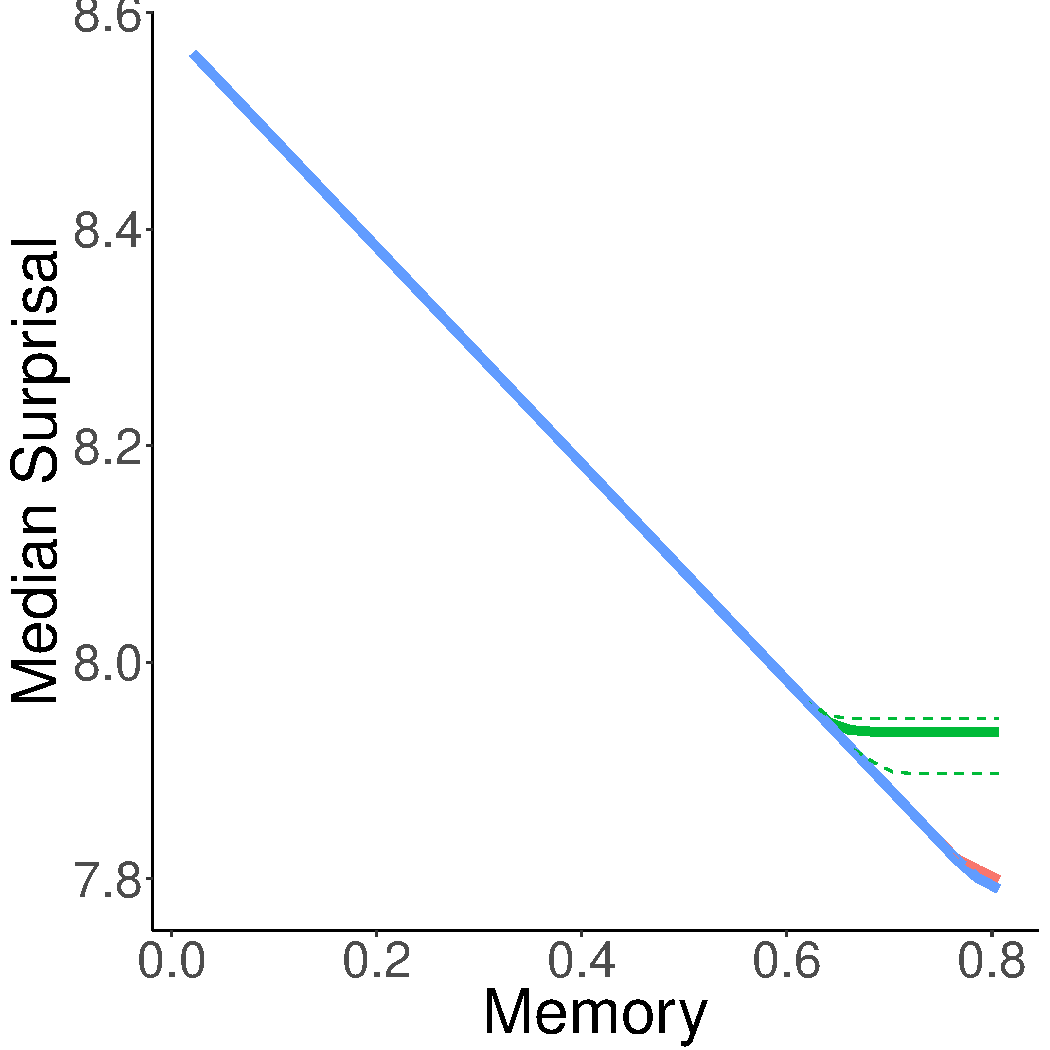
\includegraphics[width=0.25\textwidth]{../code/analyze_ngrams/visualize/figures/Croatian-listener-surprisal-memory-MEDIANS_onlyWordForms_boundedVocab.pdf} & 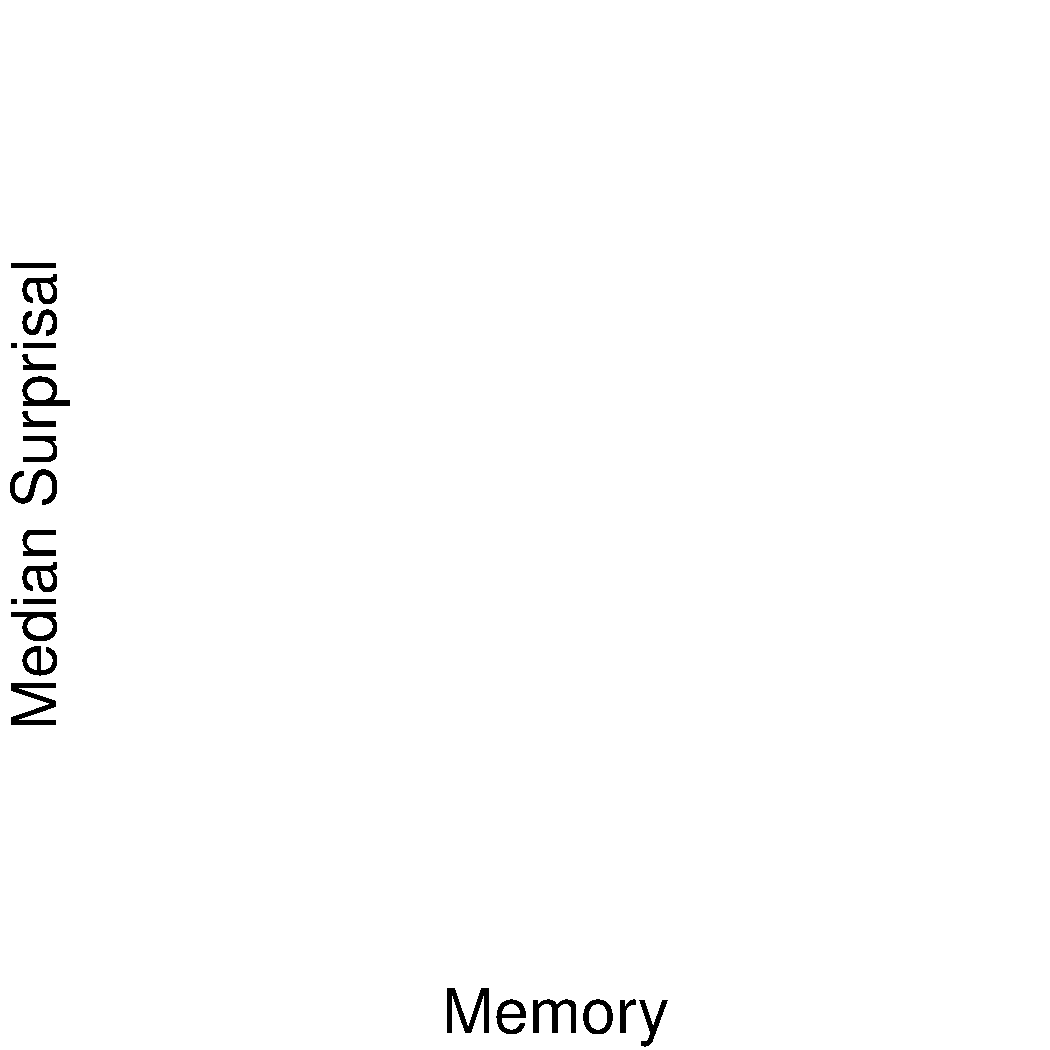
\includegraphics[width=0.25\textwidth]{../code/analyze_ngrams/visualize/figures/Czech-listener-surprisal-memory-MEDIANS_onlyWordForms_boundedVocab.pdf} & 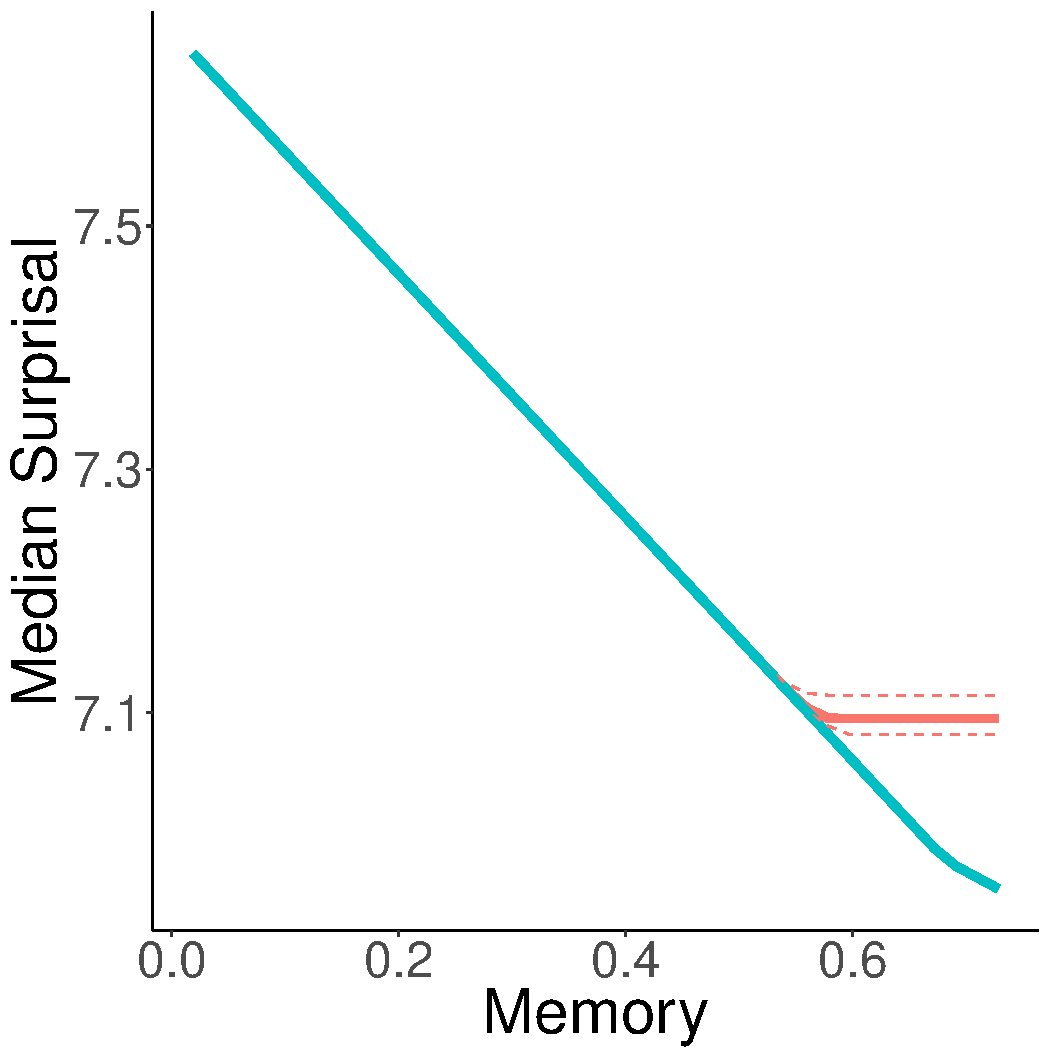
\includegraphics[width=0.25\textwidth]{../code/analyze_ngrams/visualize/figures/Danish-listener-surprisal-memory-MEDIANS_onlyWordForms_boundedVocab.pdf} & 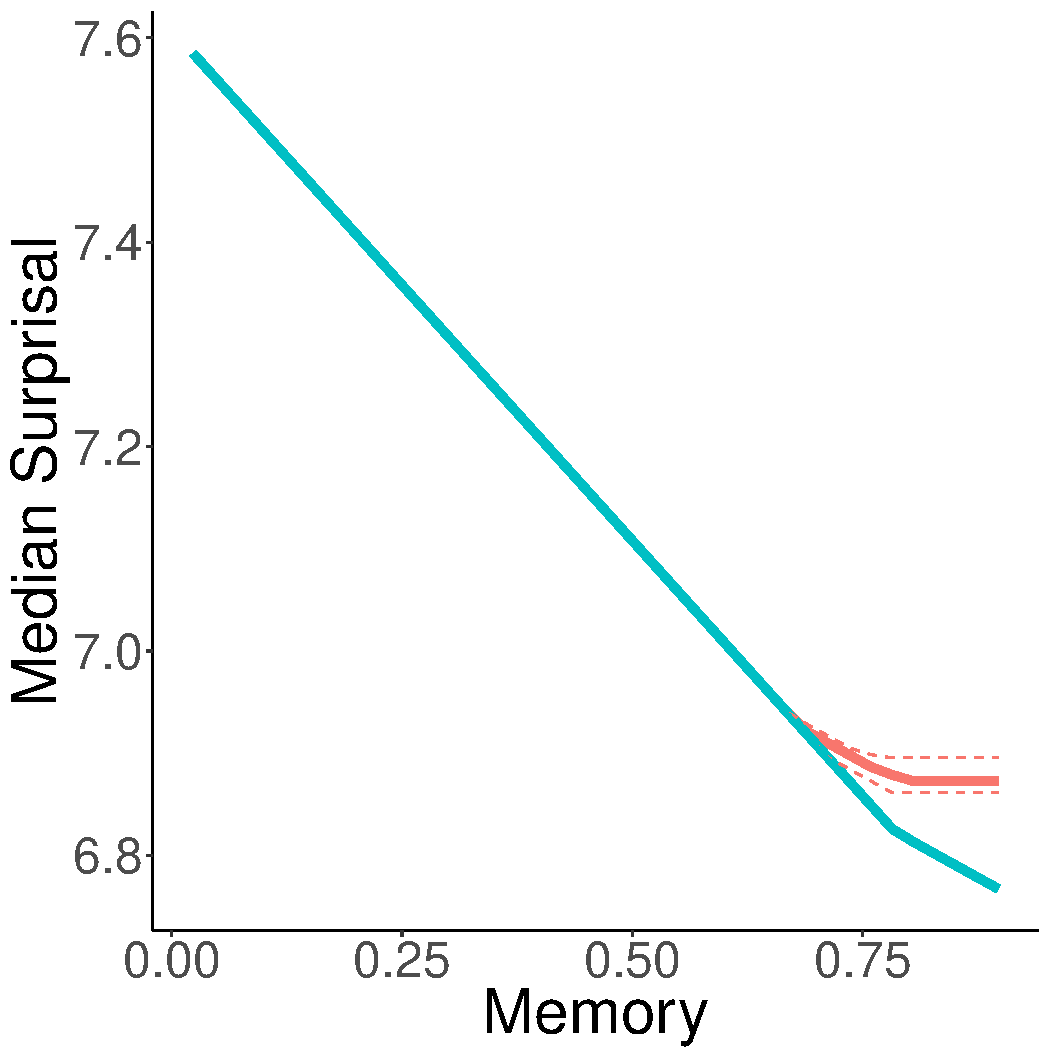
\includegraphics[width=0.25\textwidth]{../code/analyze_ngrams/visualize/figures/Dutch-listener-surprisal-memory-MEDIANS_onlyWordForms_boundedVocab.pdf}
 \\ 

Hindi & Hungarian & Japanese & Norwegian
 \\ 
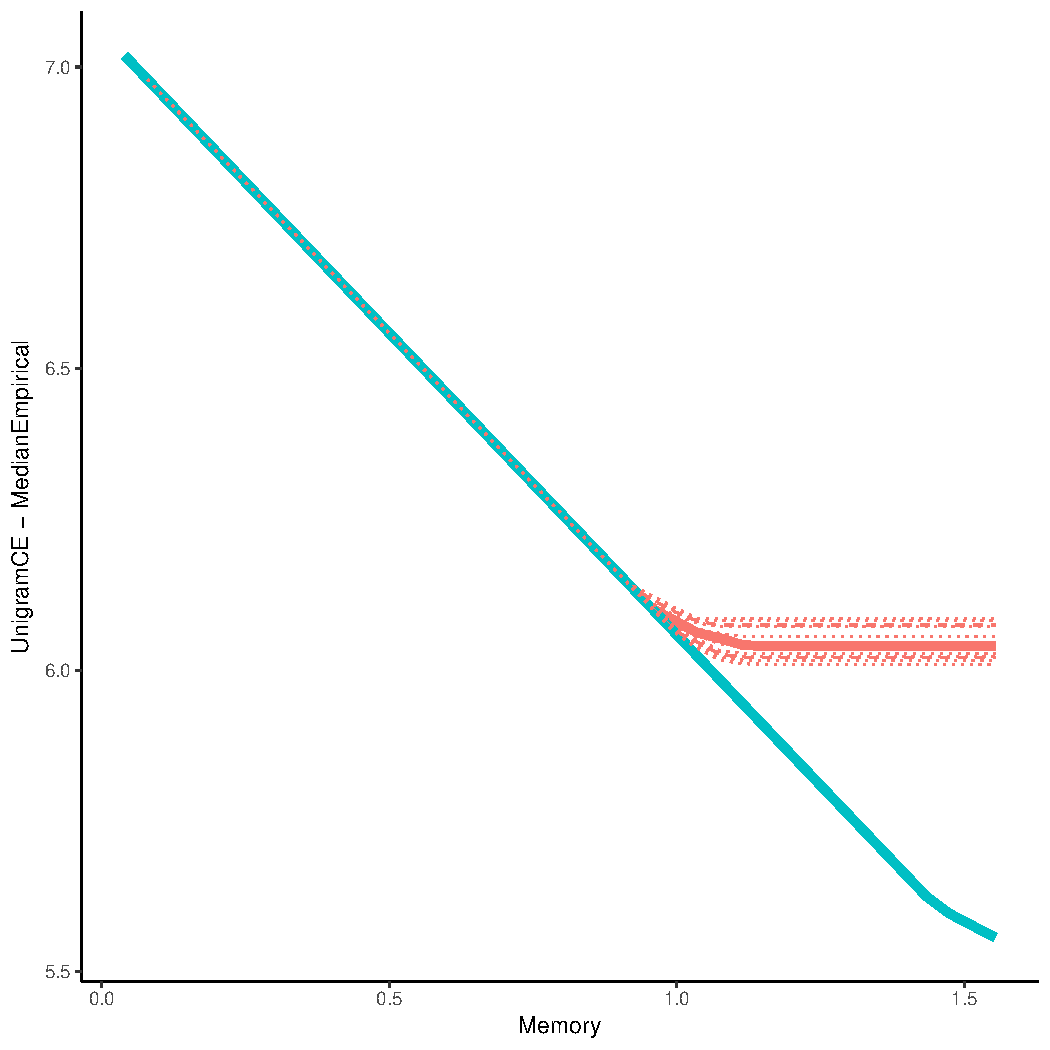
\includegraphics[width=0.25\textwidth]{ngrams/figures/Hindi-listener-surprisal-memory-MEDIANS_QUANTILES_onlyWordForms_boundedVocab.pdf} & 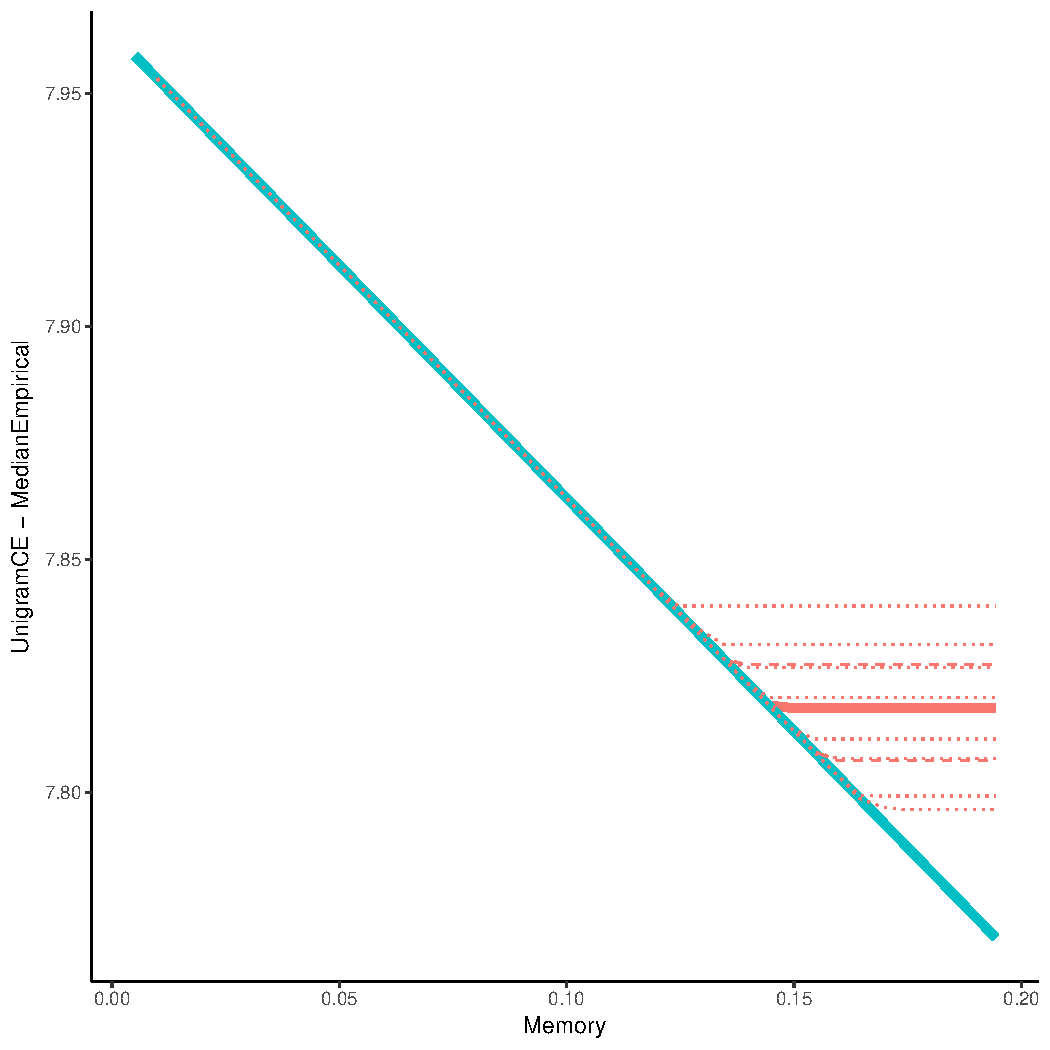
\includegraphics[width=0.25\textwidth]{ngrams/figures/Hungarian-listener-surprisal-memory-MEDIANS_QUANTILES_onlyWordForms_boundedVocab.pdf} & 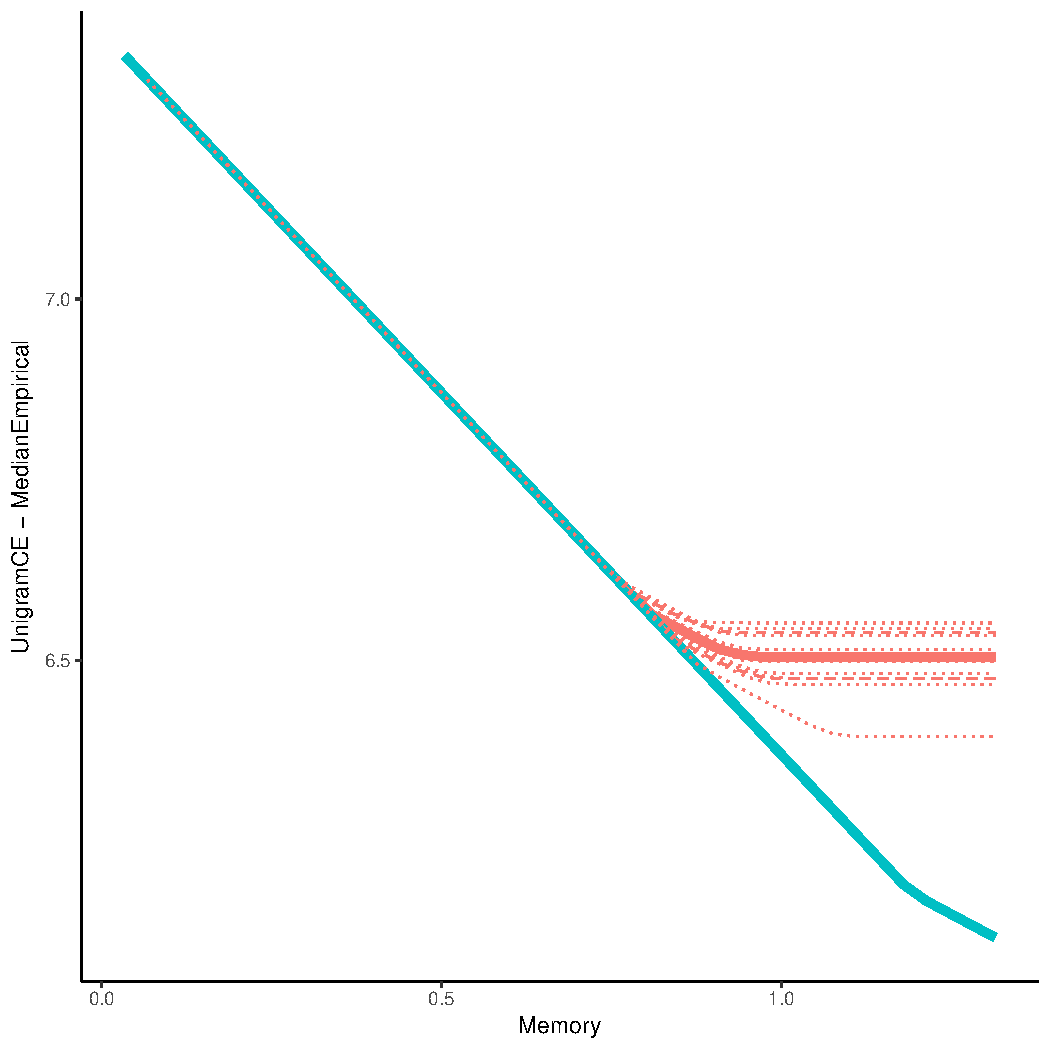
\includegraphics[width=0.25\textwidth]{ngrams/figures/Japanese-listener-surprisal-memory-MEDIANS_QUANTILES_onlyWordForms_boundedVocab.pdf} & 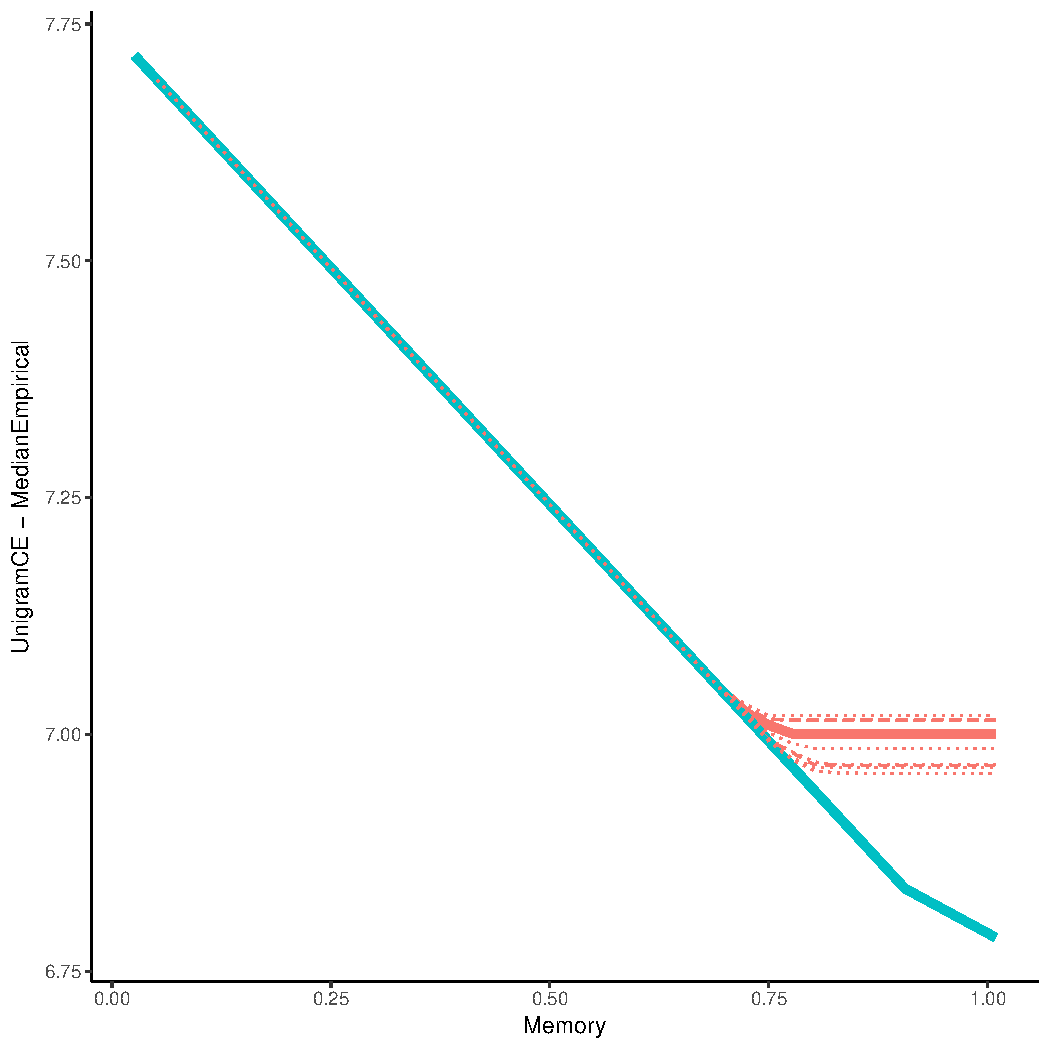
\includegraphics[width=0.25\textwidth]{ngrams/figures/Norwegian-listener-surprisal-memory-MEDIANS_QUANTILES_onlyWordForms_boundedVocab.pdf}
 \\ 
Polish & Romanian & Slovak & Slovenian
 \\ 
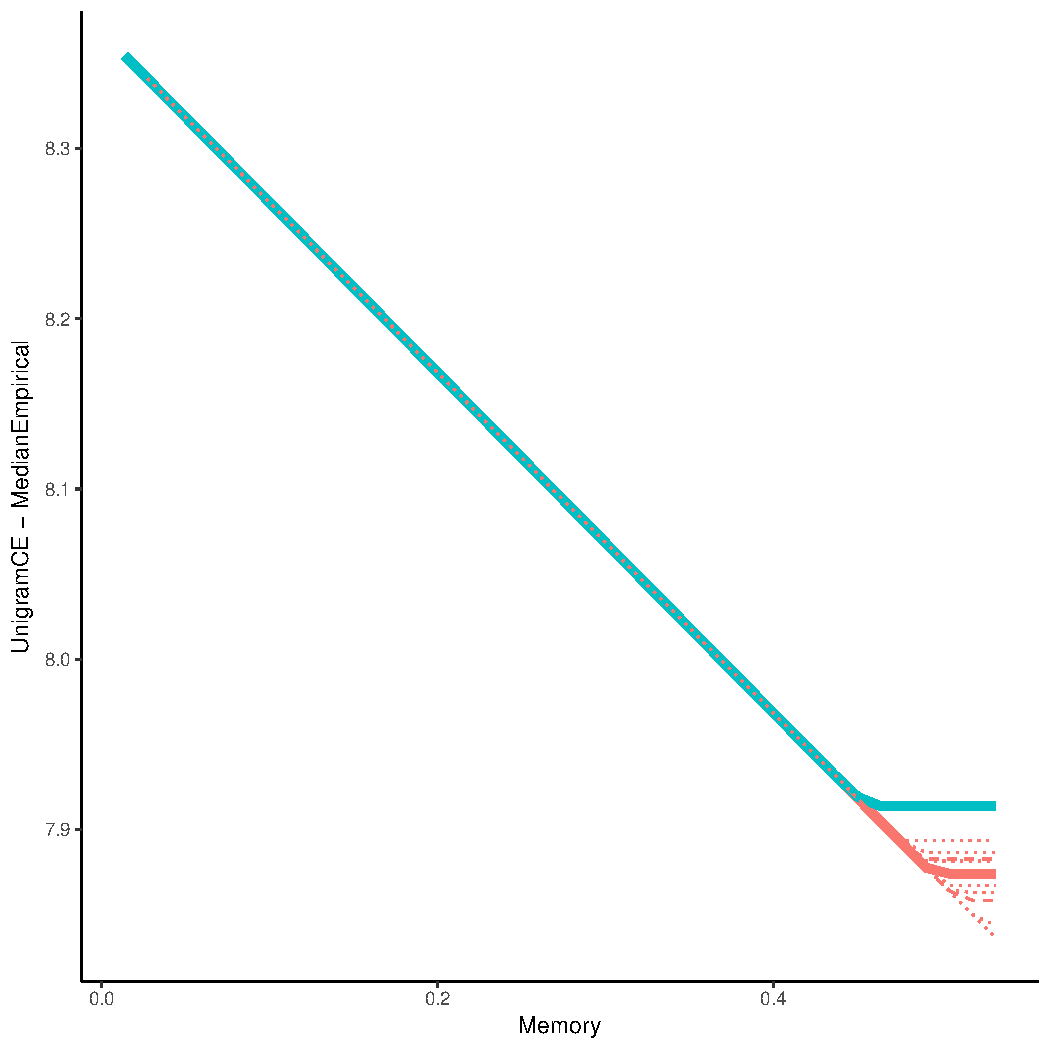
\includegraphics[width=0.25\textwidth]{ngrams/figures/Polish-listener-surprisal-memory-MEDIANS_QUANTILES_onlyWordForms_boundedVocab.pdf} & 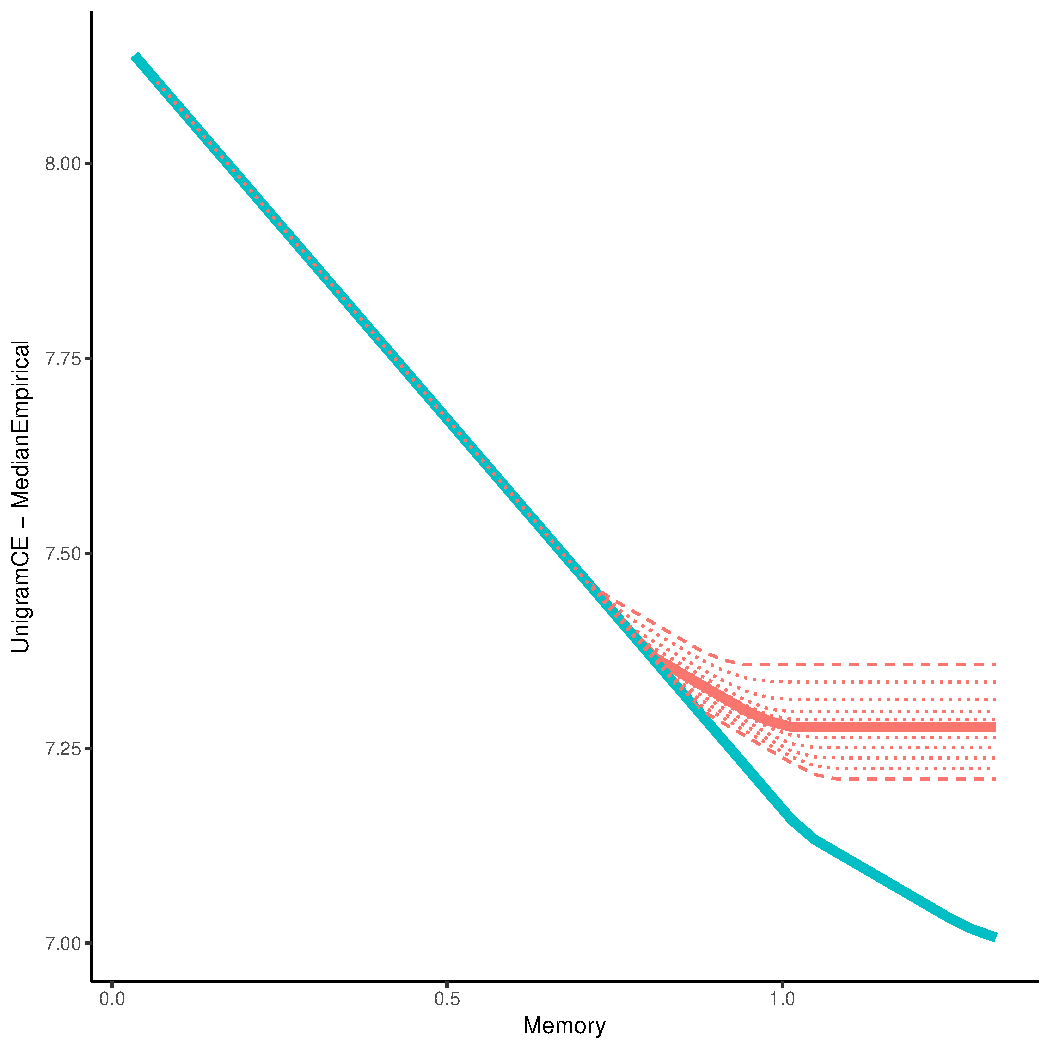
\includegraphics[width=0.25\textwidth]{ngrams/figures/Romanian-listener-surprisal-memory-MEDIANS_QUANTILES_onlyWordForms_boundedVocab.pdf} & 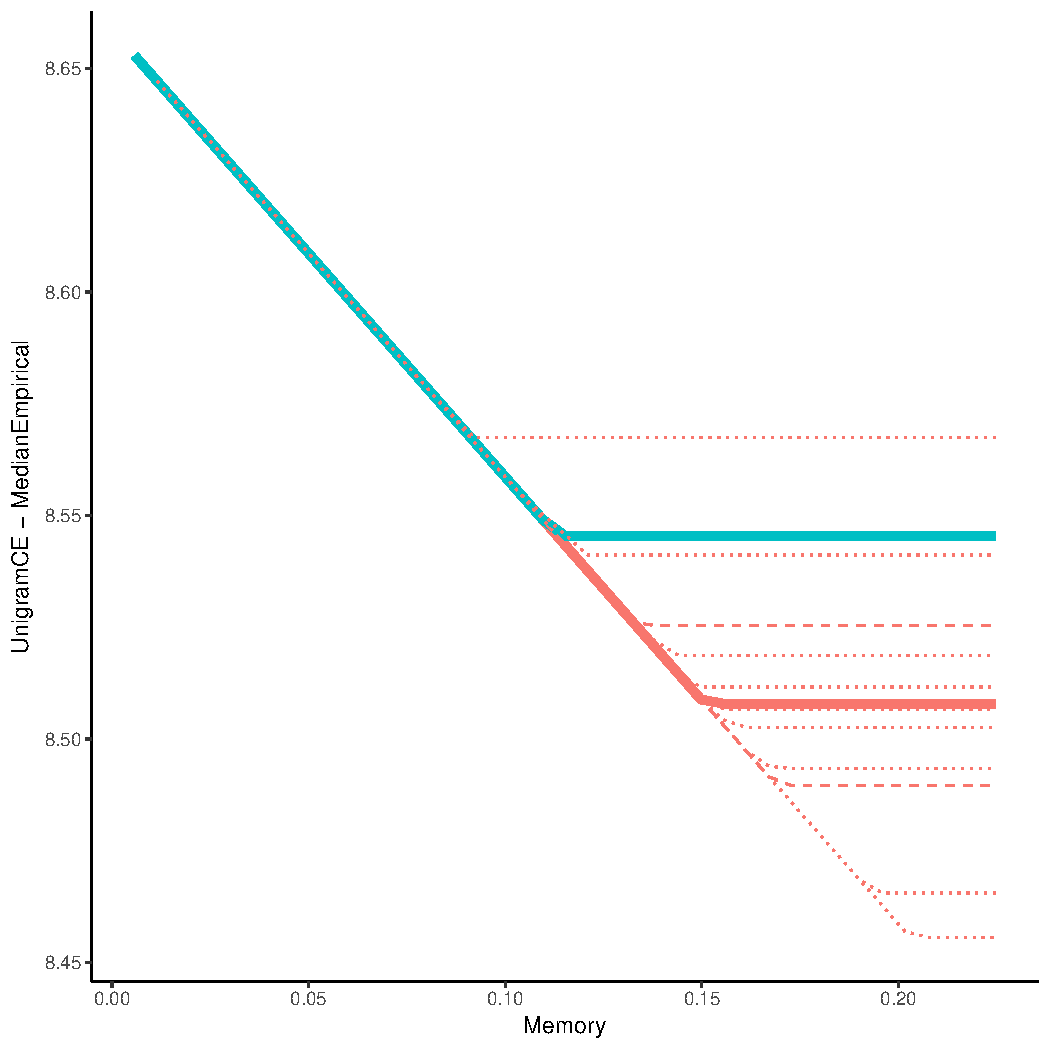
\includegraphics[width=0.25\textwidth]{ngrams/figures/Slovak-listener-surprisal-memory-MEDIANS_QUANTILES_onlyWordForms_boundedVocab.pdf} & 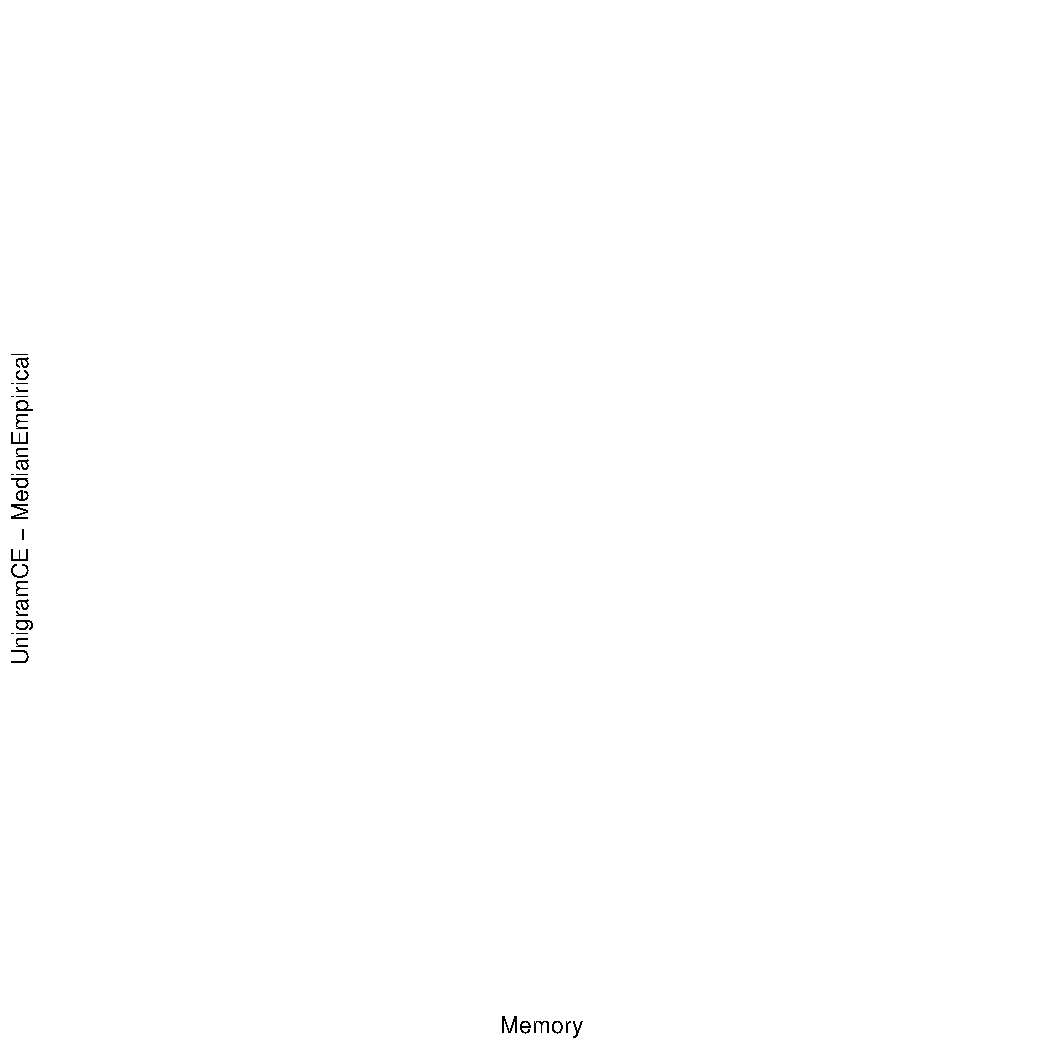
\includegraphics[width=0.25\textwidth]{ngrams/figures/Slovenian-listener-surprisal-memory-MEDIANS_QUANTILES_onlyWordForms_boundedVocab.pdf}
 \\ 
Spanish & Swedish &  & 
 \\ 
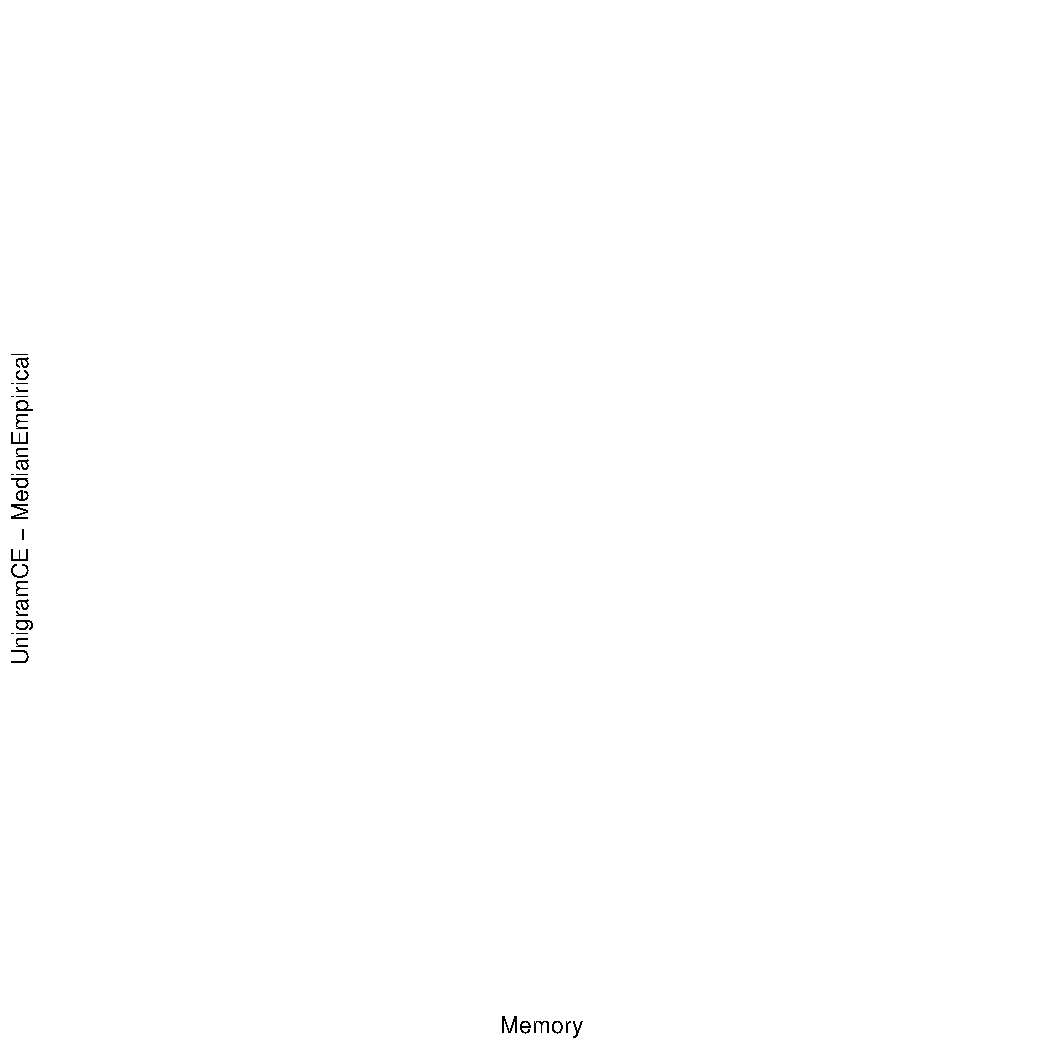
\includegraphics[width=0.25\textwidth]{ngrams/figures/Spanish-listener-surprisal-memory-MEDIANS_QUANTILES_onlyWordForms_boundedVocab.pdf} & 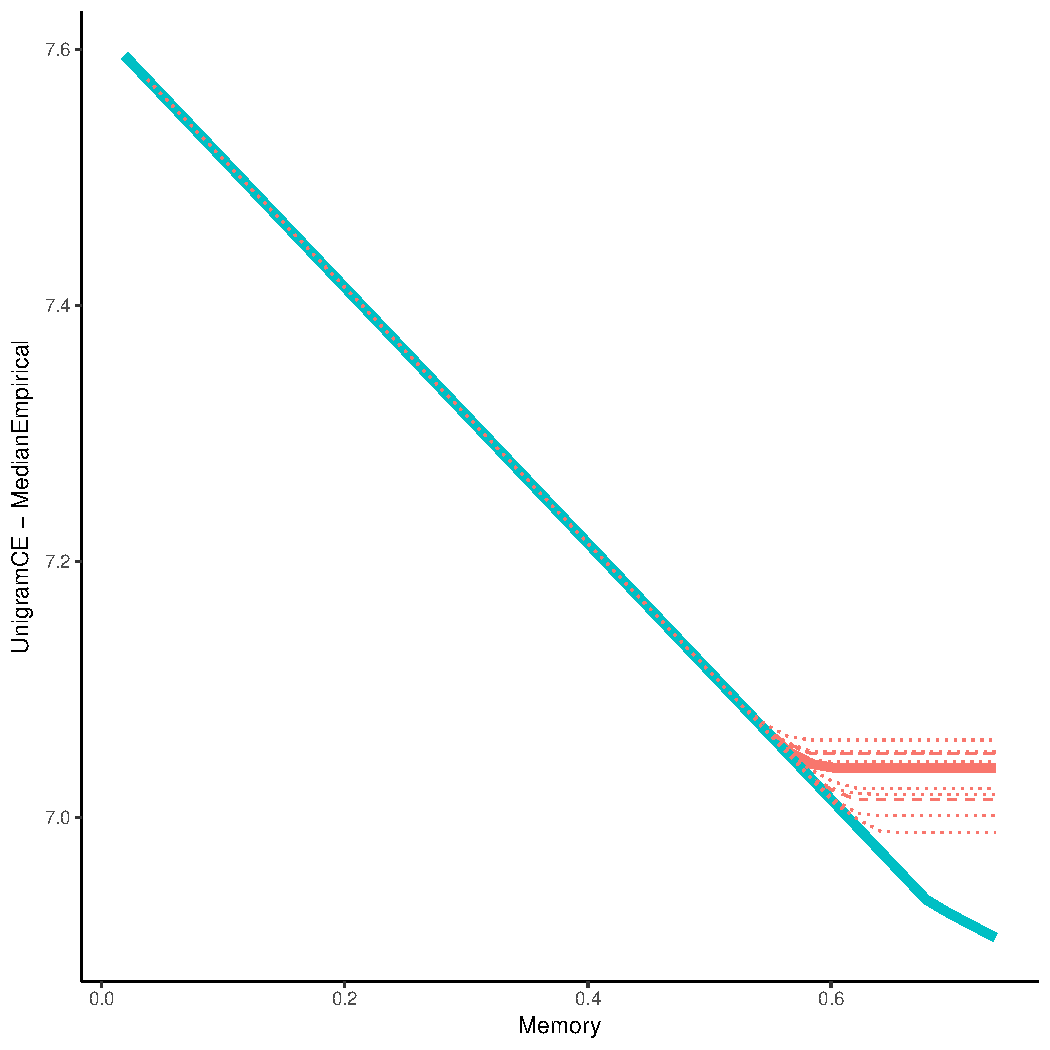
\includegraphics[width=0.25\textwidth]{ngrams/figures/Swedish-listener-surprisal-memory-MEDIANS_QUANTILES_onlyWordForms_boundedVocab.pdf} &  & 
 \\ 

Kurmanji & Latvian & Maltese & Naija
 \\ 
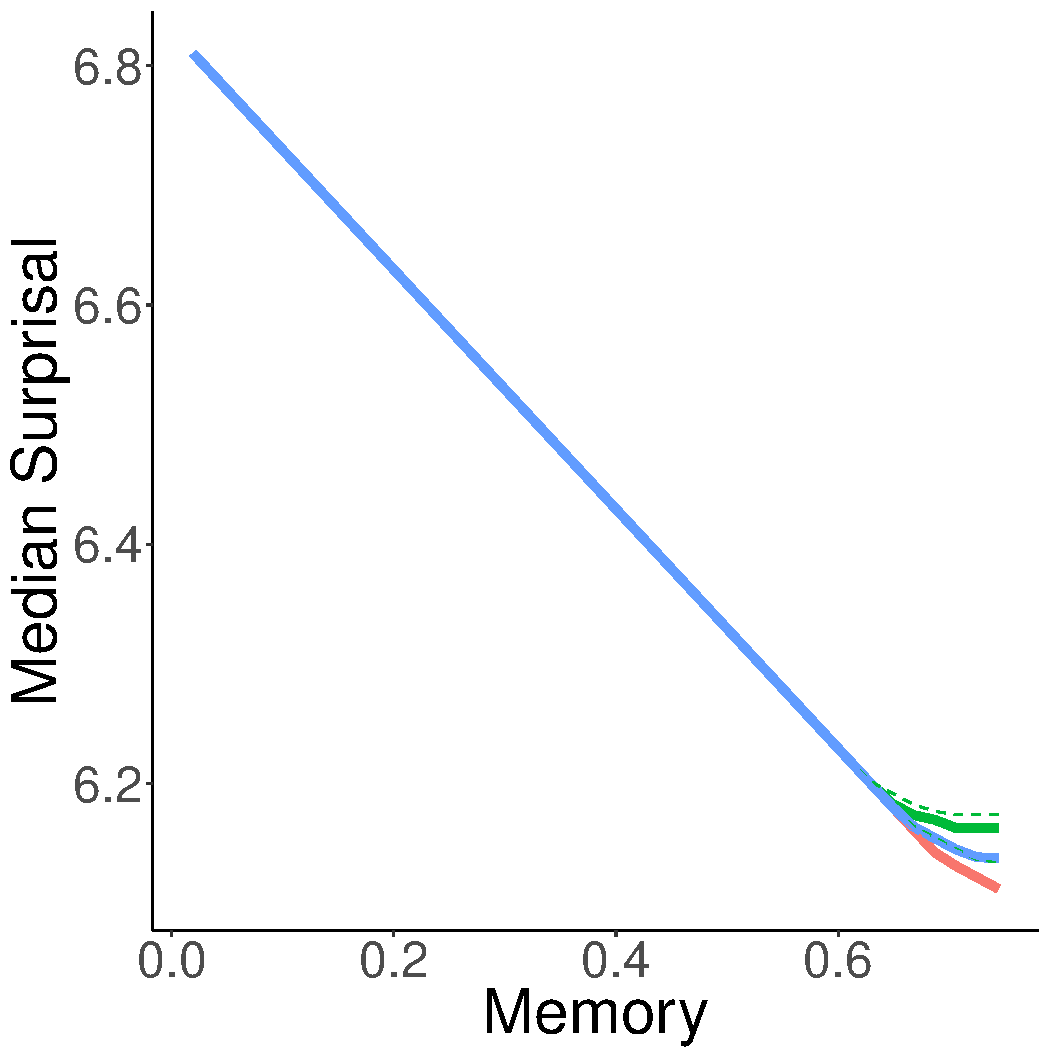
\includegraphics[width=0.25\textwidth]{../code/analyze_ngrams/visualize/figures/Kurmanji-Adap-listener-surprisal-memory-MEDIANS_onlyWordForms_boundedVocab.pdf} & 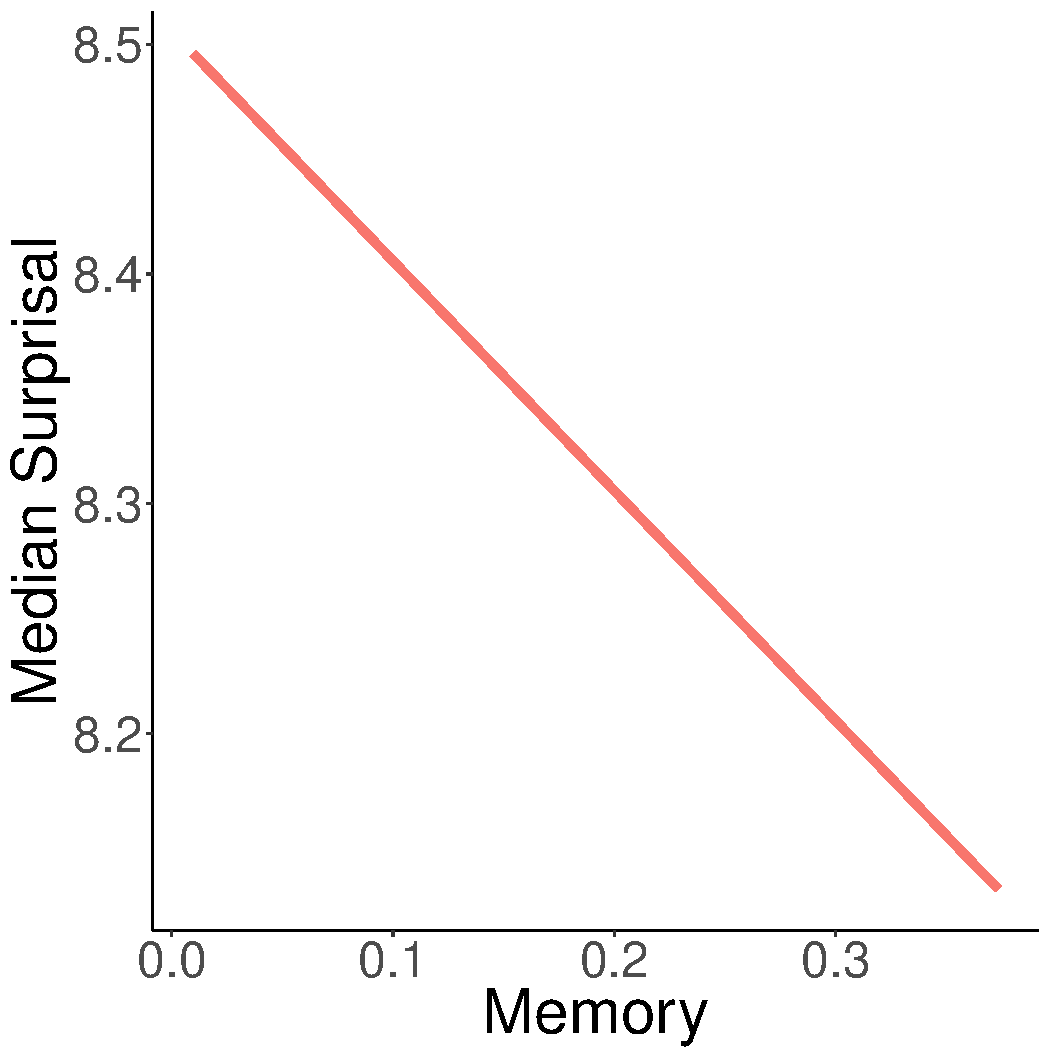
\includegraphics[width=0.25\textwidth]{../code/analyze_ngrams/visualize/figures/Latvian-listener-surprisal-memory-MEDIANS_onlyWordForms_boundedVocab.pdf} & 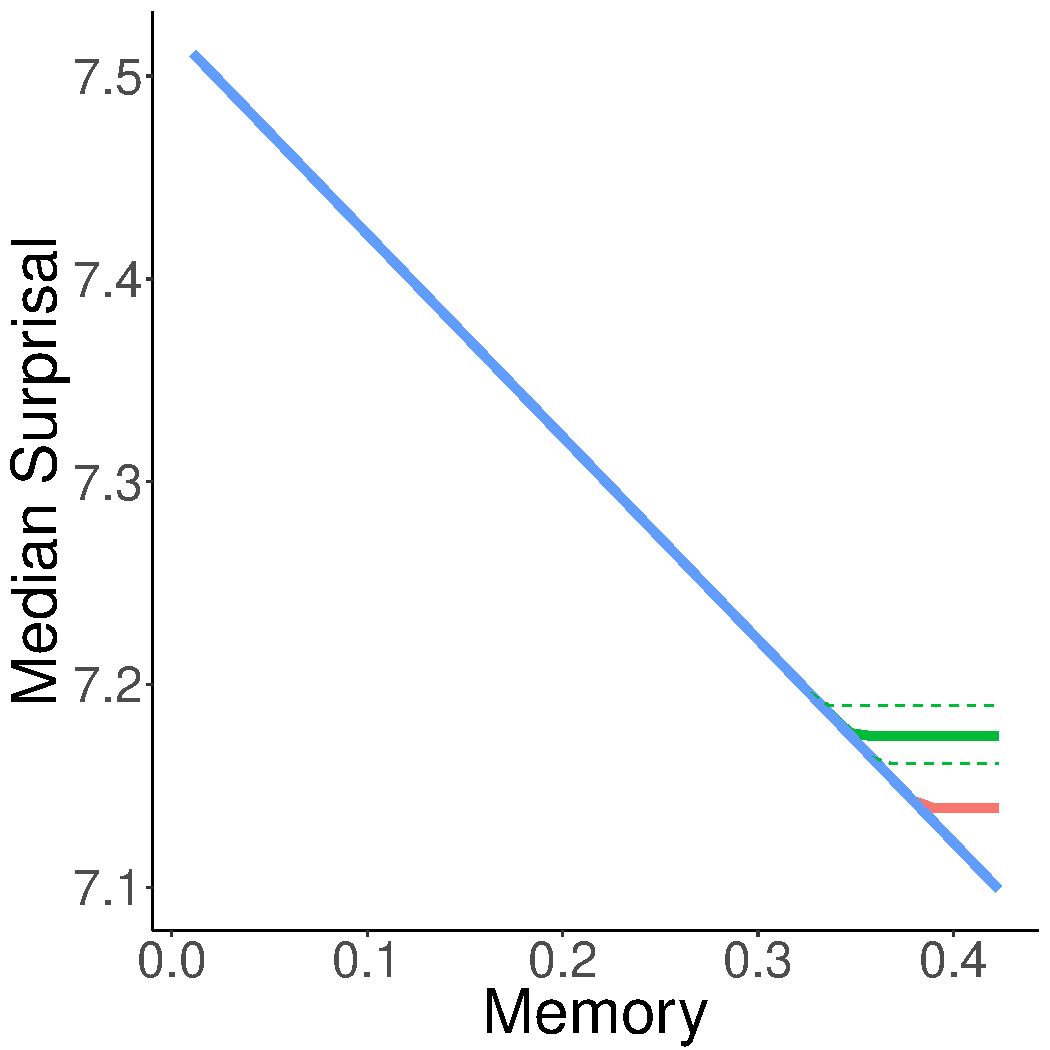
\includegraphics[width=0.25\textwidth]{../code/analyze_ngrams/visualize/figures/Maltese-listener-surprisal-memory-MEDIANS_onlyWordForms_boundedVocab.pdf} & 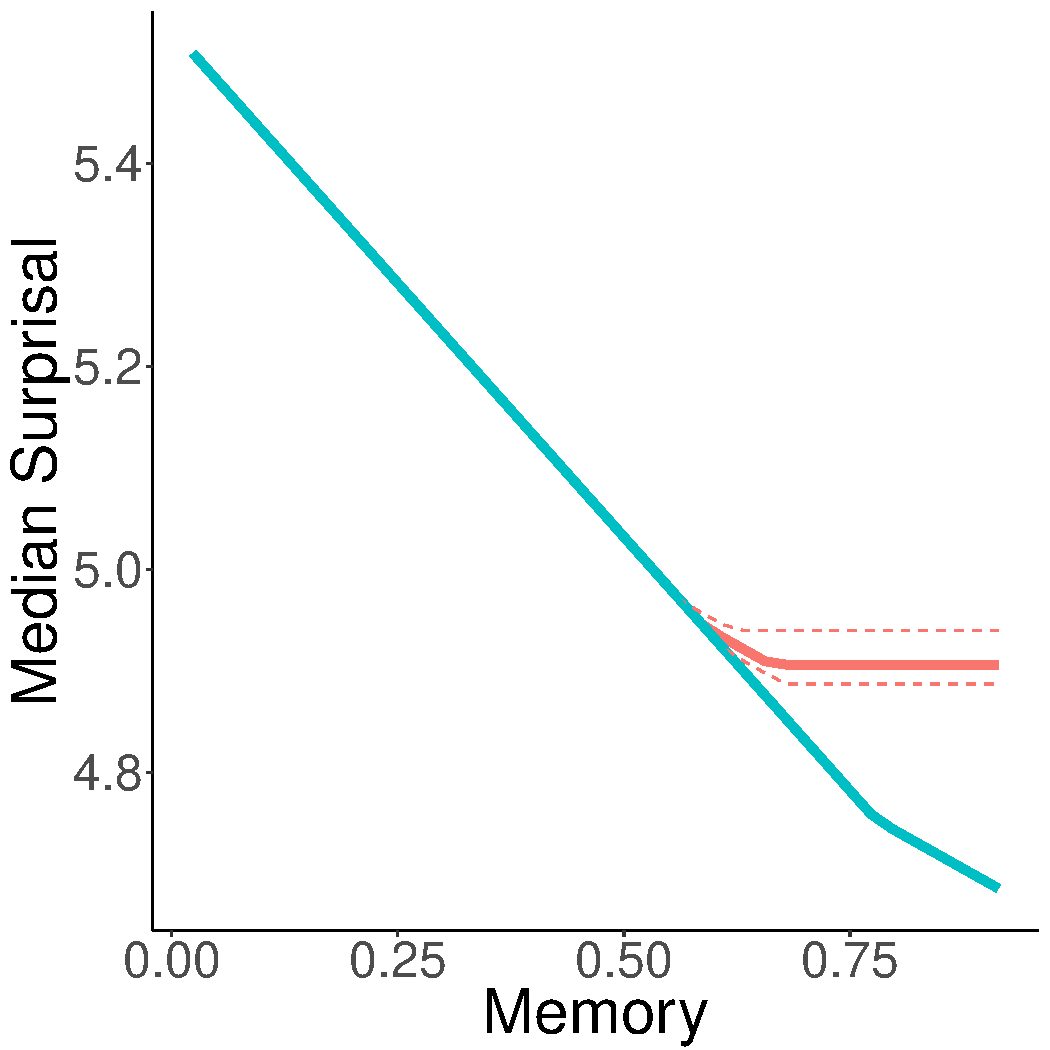
\includegraphics[width=0.25\textwidth]{../code/analyze_ngrams/visualize/figures/Naija-Adap-listener-surprisal-memory-MEDIANS_onlyWordForms_boundedVocab.pdf}
 \\ 
North Sami & Norwegian & Persian & Polish
 \\ 
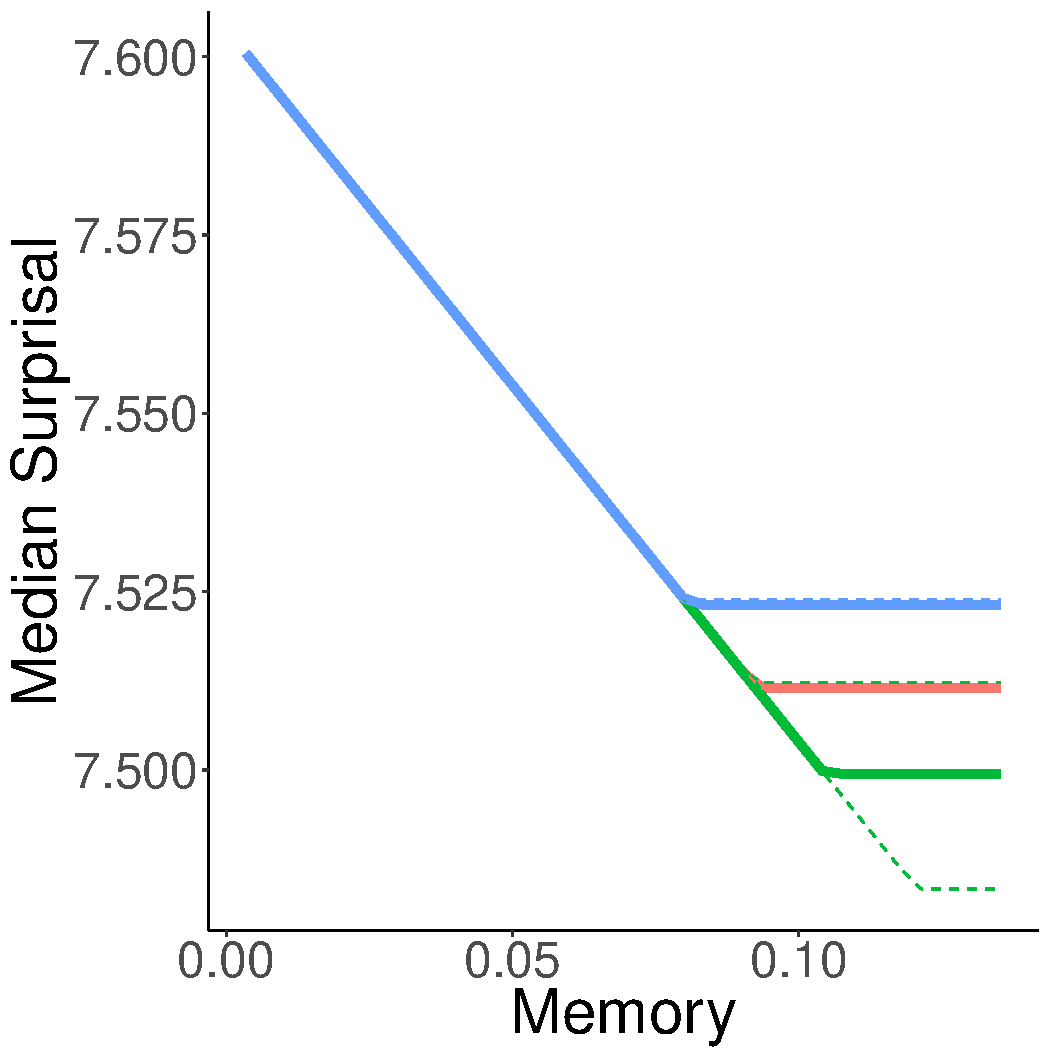
\includegraphics[width=0.25\textwidth]{../code/analyze_ngrams/visualize/figures/North_Sami-listener-surprisal-memory-MEDIANS_onlyWordForms_boundedVocab.pdf} & 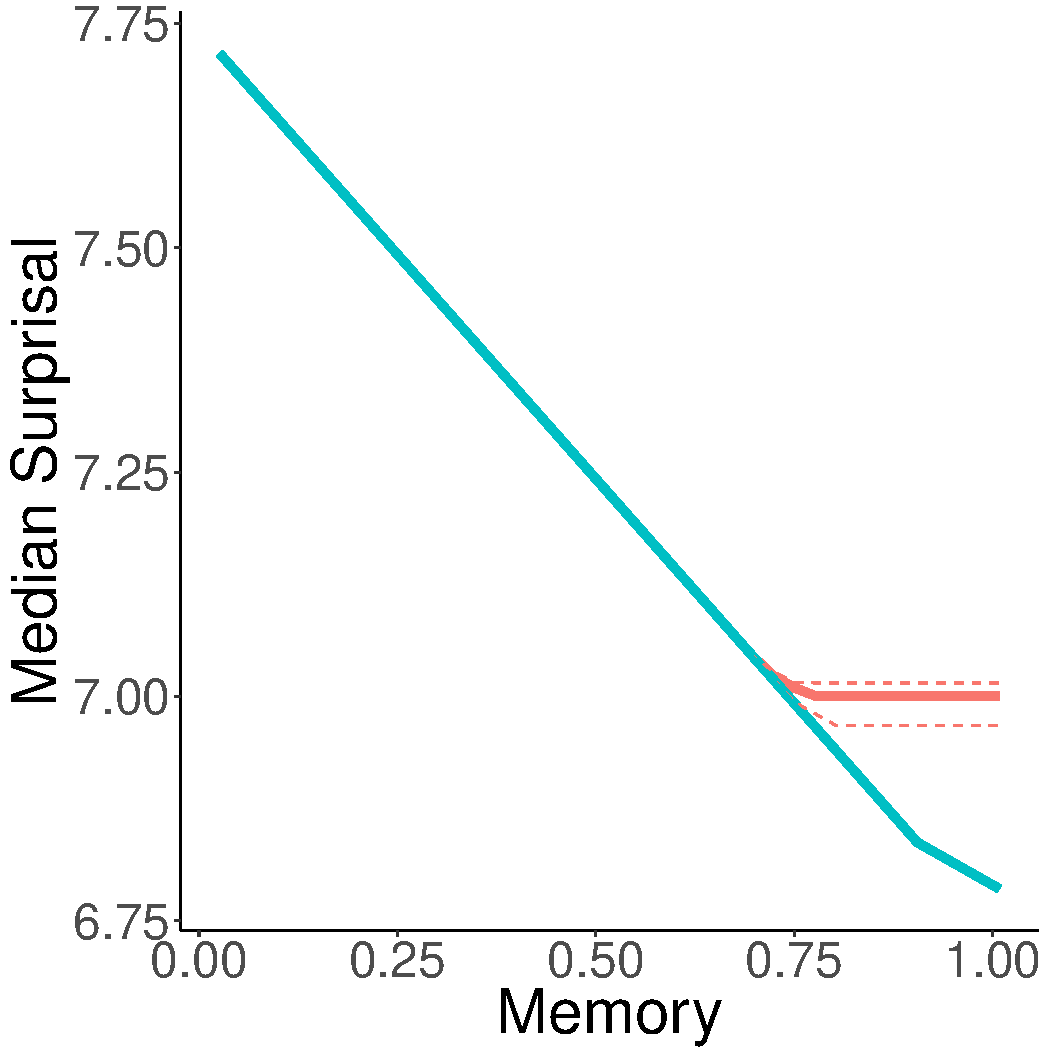
\includegraphics[width=0.25\textwidth]{../code/analyze_ngrams/visualize/figures/Norwegian-listener-surprisal-memory-MEDIANS_onlyWordForms_boundedVocab.pdf} & 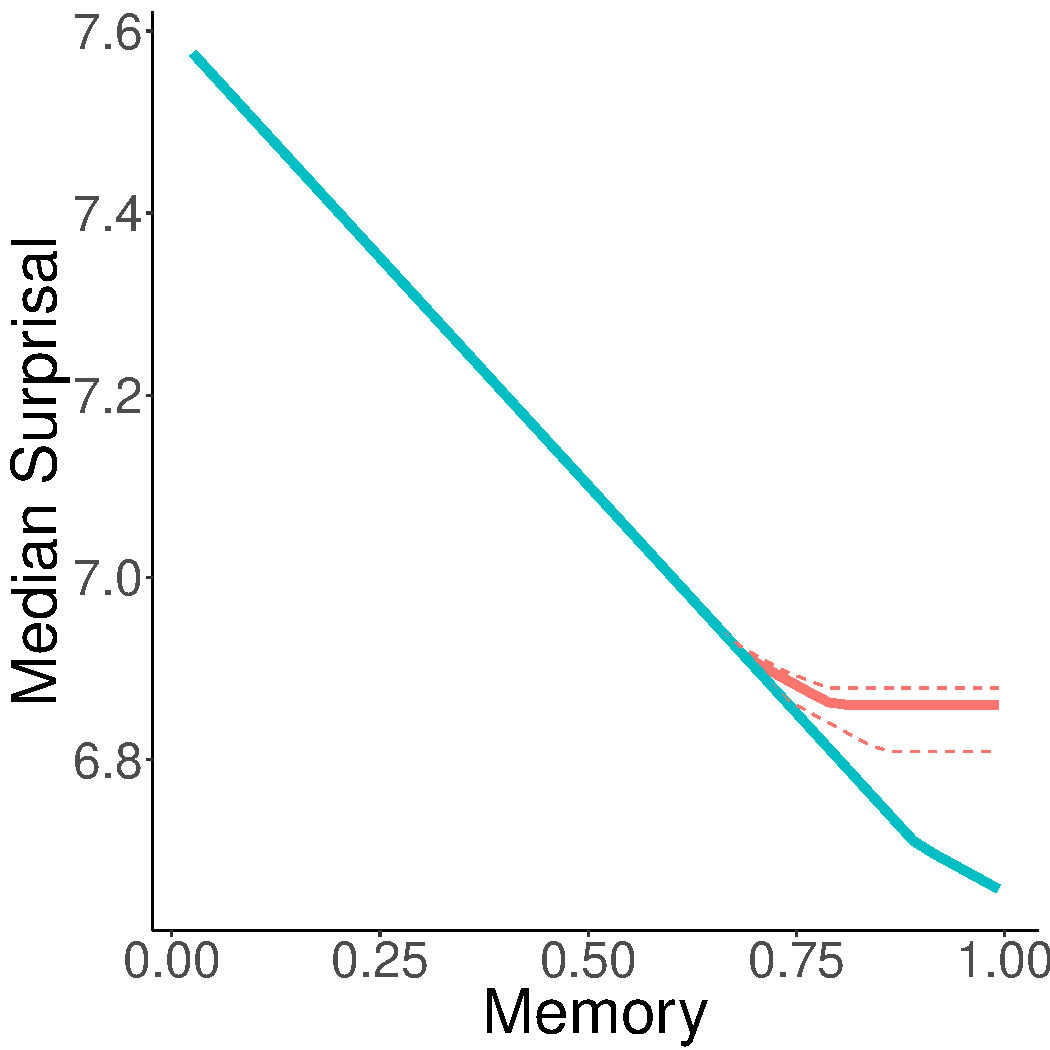
\includegraphics[width=0.25\textwidth]{../code/analyze_ngrams/visualize/figures/Persian-listener-surprisal-memory-MEDIANS_onlyWordForms_boundedVocab.pdf} & 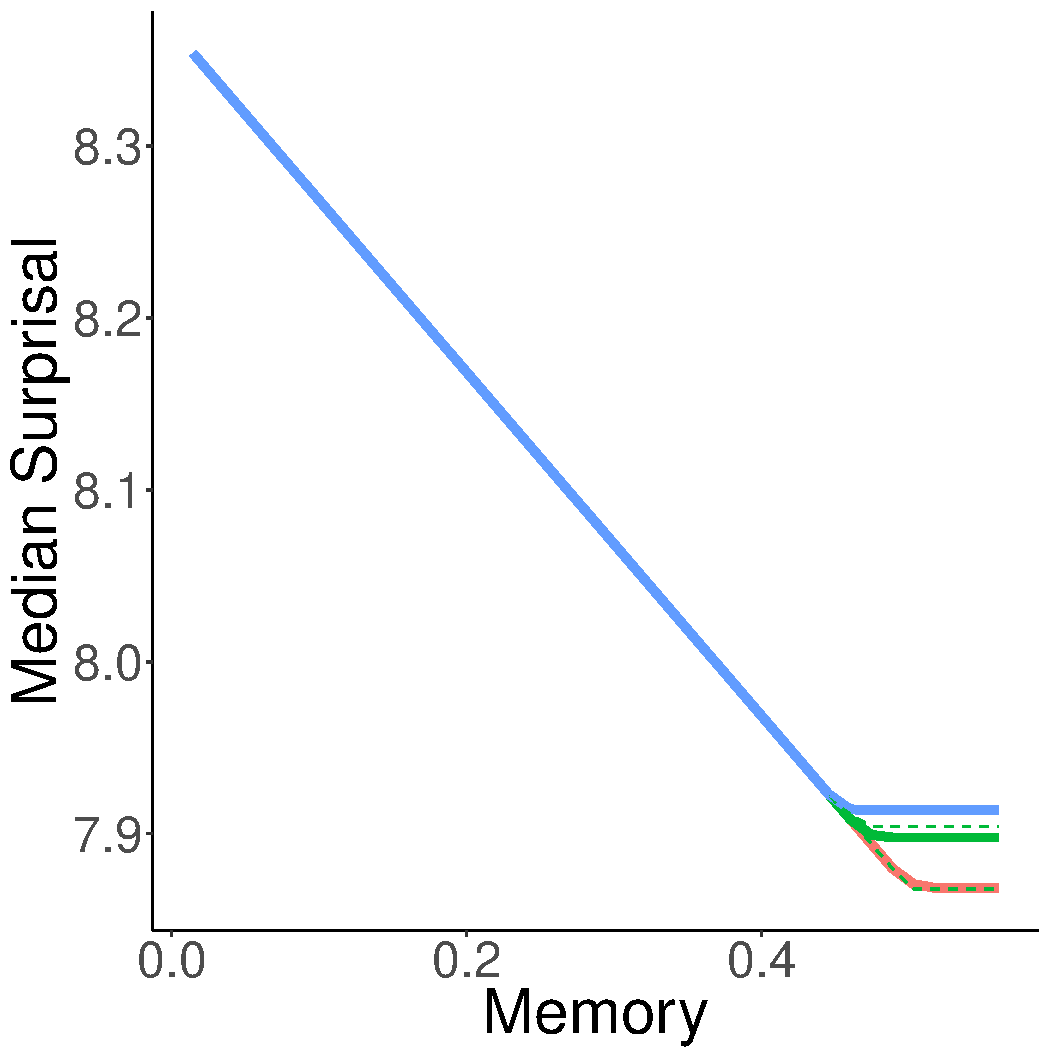
\includegraphics[width=0.25\textwidth]{../code/analyze_ngrams/visualize/figures/Polish-listener-surprisal-memory-MEDIANS_onlyWordForms_boundedVocab.pdf}
 \\ 
Portuguese & Romanian & Russian & Serbian
 \\ 
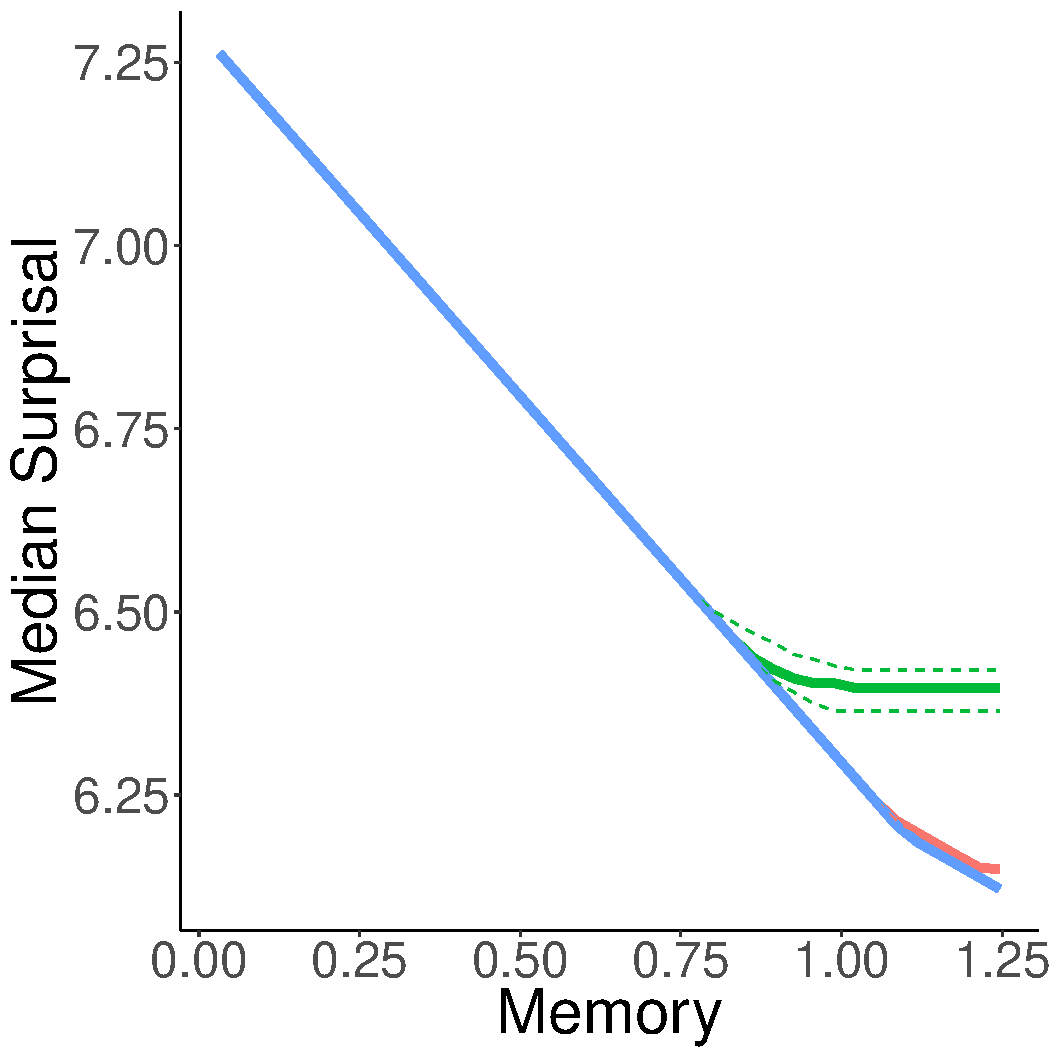
\includegraphics[width=0.25\textwidth]{../code/analyze_ngrams/visualize/figures/Portuguese-listener-surprisal-memory-MEDIANS_onlyWordForms_boundedVocab.pdf} & 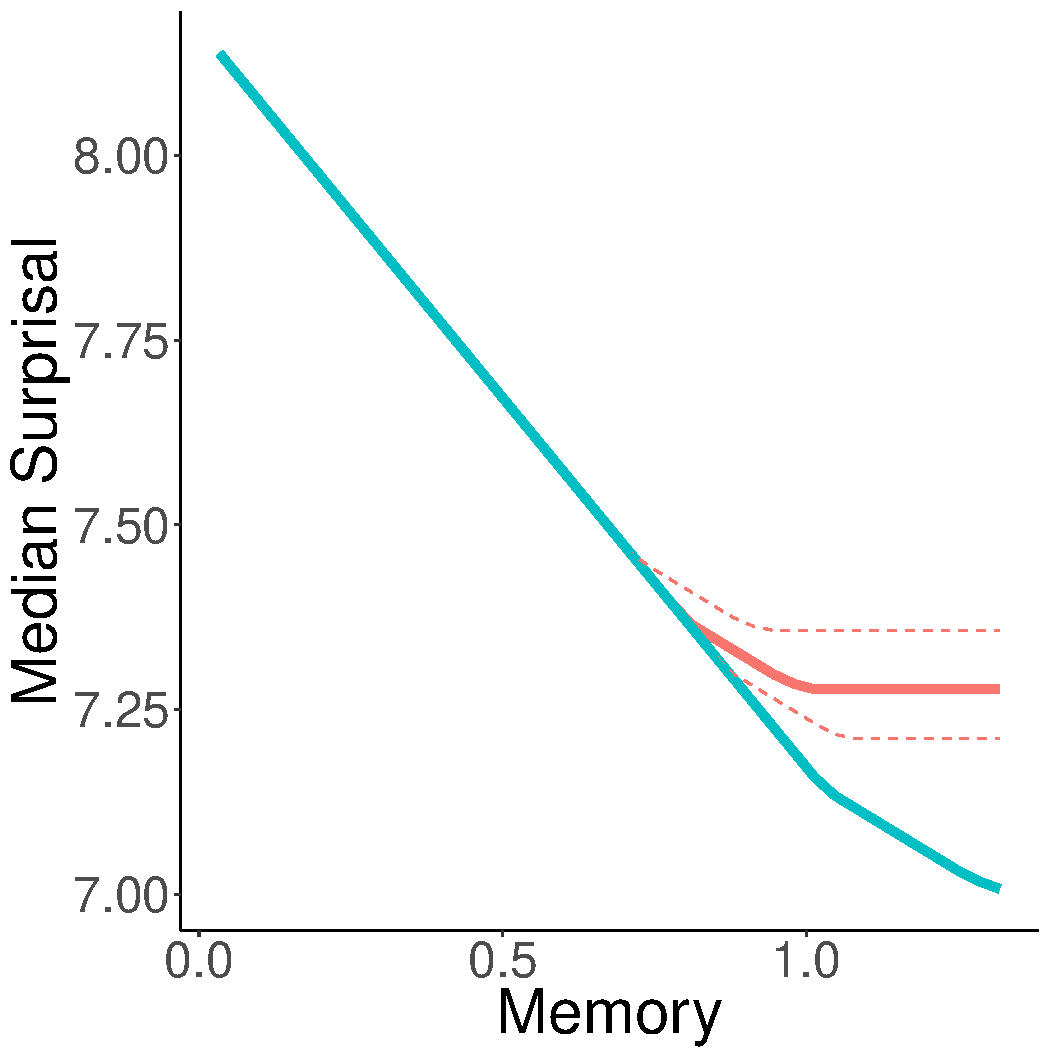
\includegraphics[width=0.25\textwidth]{../code/analyze_ngrams/visualize/figures/Romanian-listener-surprisal-memory-MEDIANS_onlyWordForms_boundedVocab.pdf} & 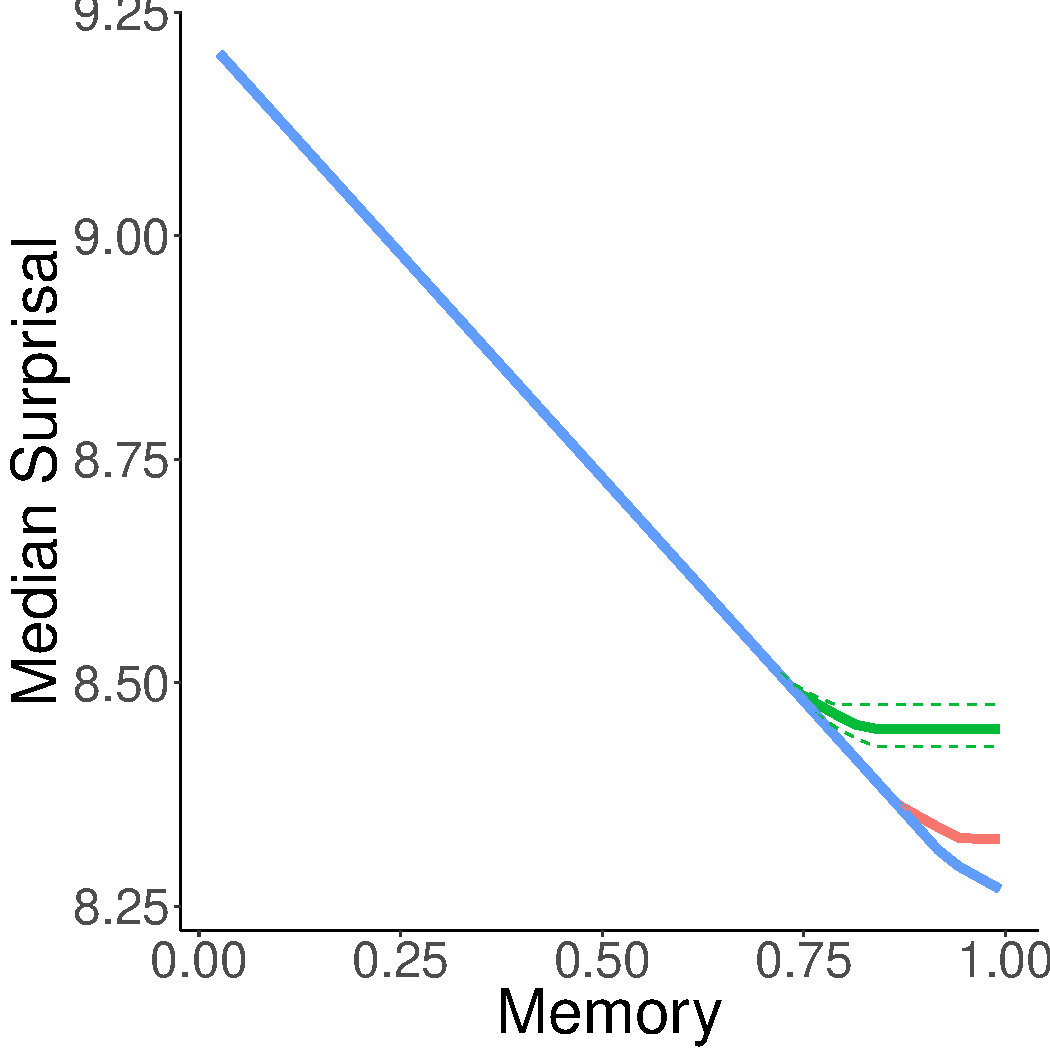
\includegraphics[width=0.25\textwidth]{../code/analyze_ngrams/visualize/figures/Russian-listener-surprisal-memory-MEDIANS_onlyWordForms_boundedVocab.pdf} & 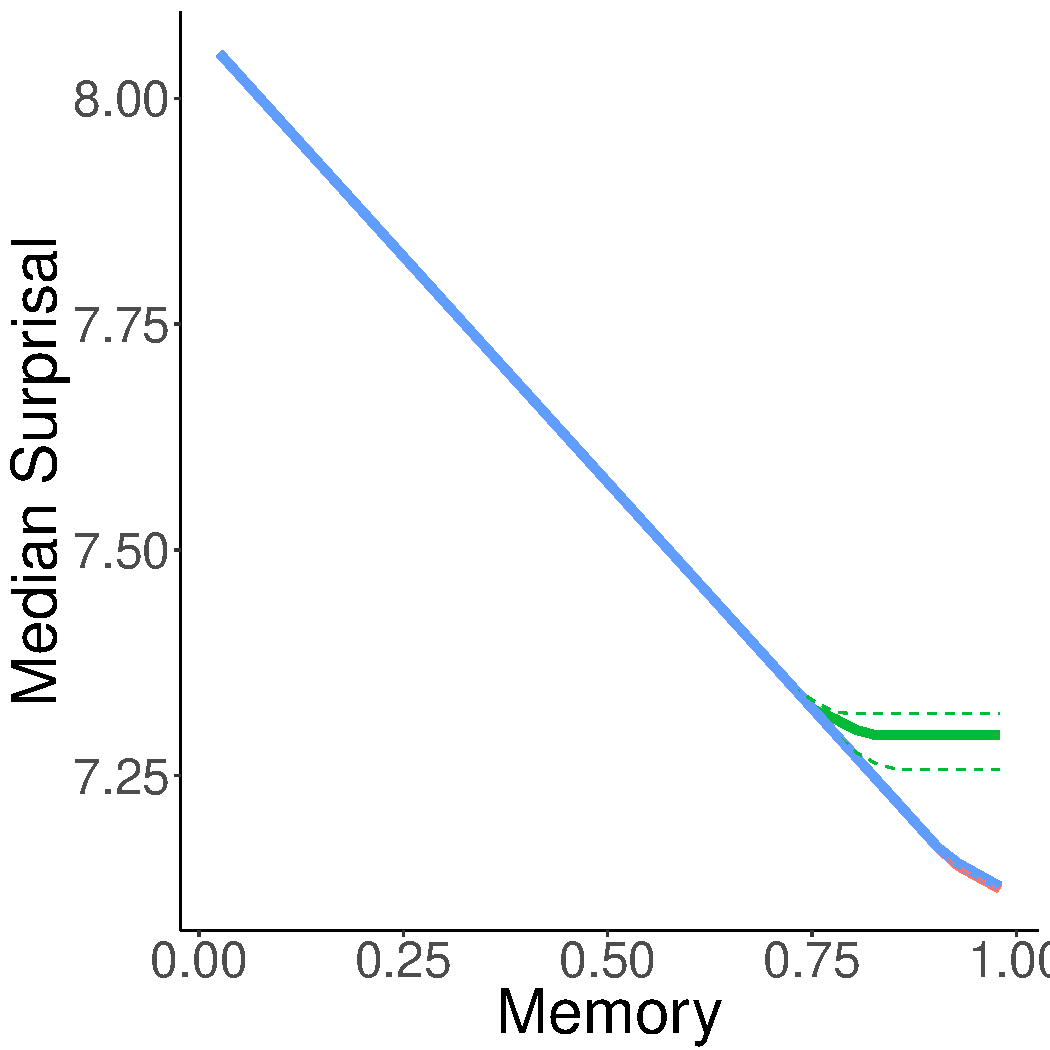
\includegraphics[width=0.25\textwidth]{../code/analyze_ngrams/visualize/figures/Serbian-listener-surprisal-memory-MEDIANS_onlyWordForms_boundedVocab.pdf}
 \\ 
Slovak & Slovenian & Spanish & Swedish
 \\ 
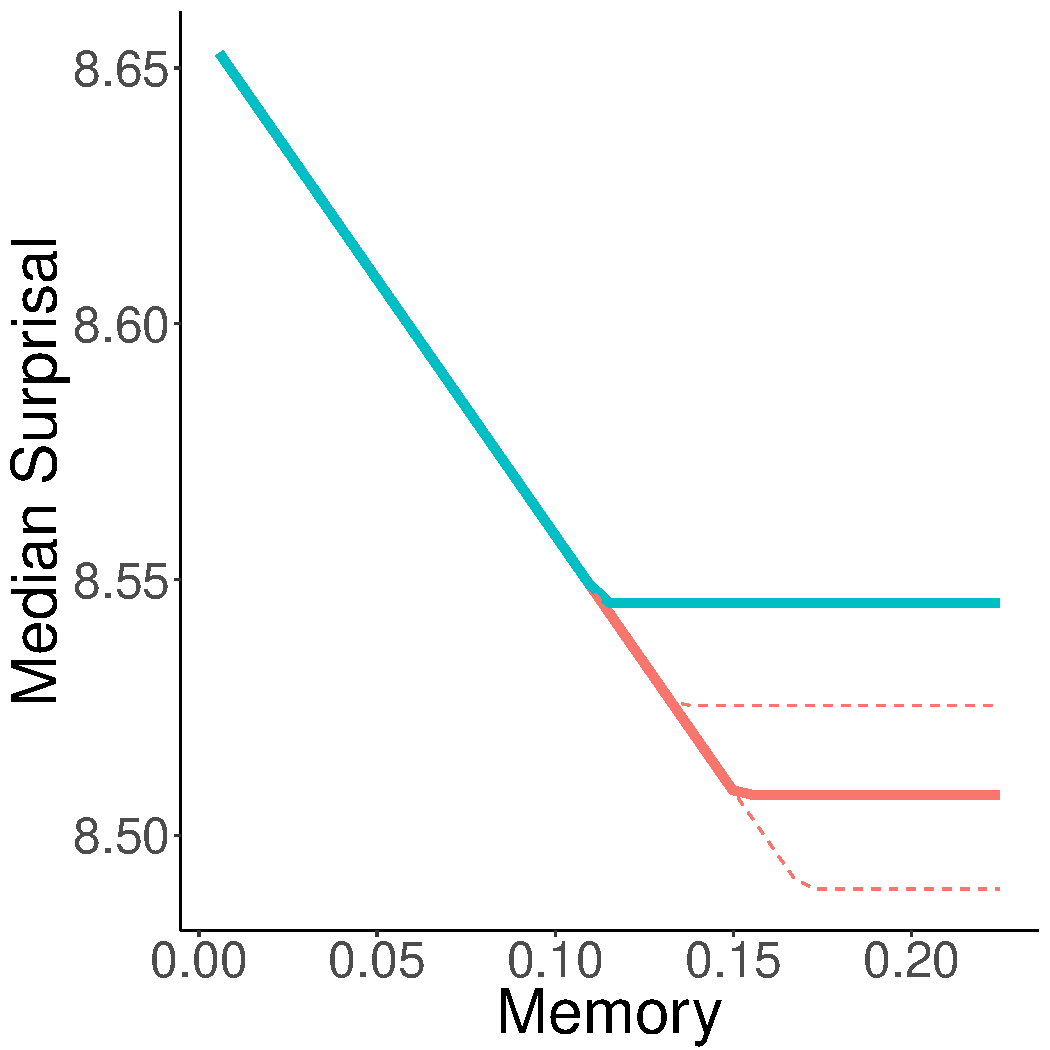
\includegraphics[width=0.25\textwidth]{../code/analyze_ngrams/visualize/figures/Slovak-listener-surprisal-memory-MEDIANS_onlyWordForms_boundedVocab.pdf} & 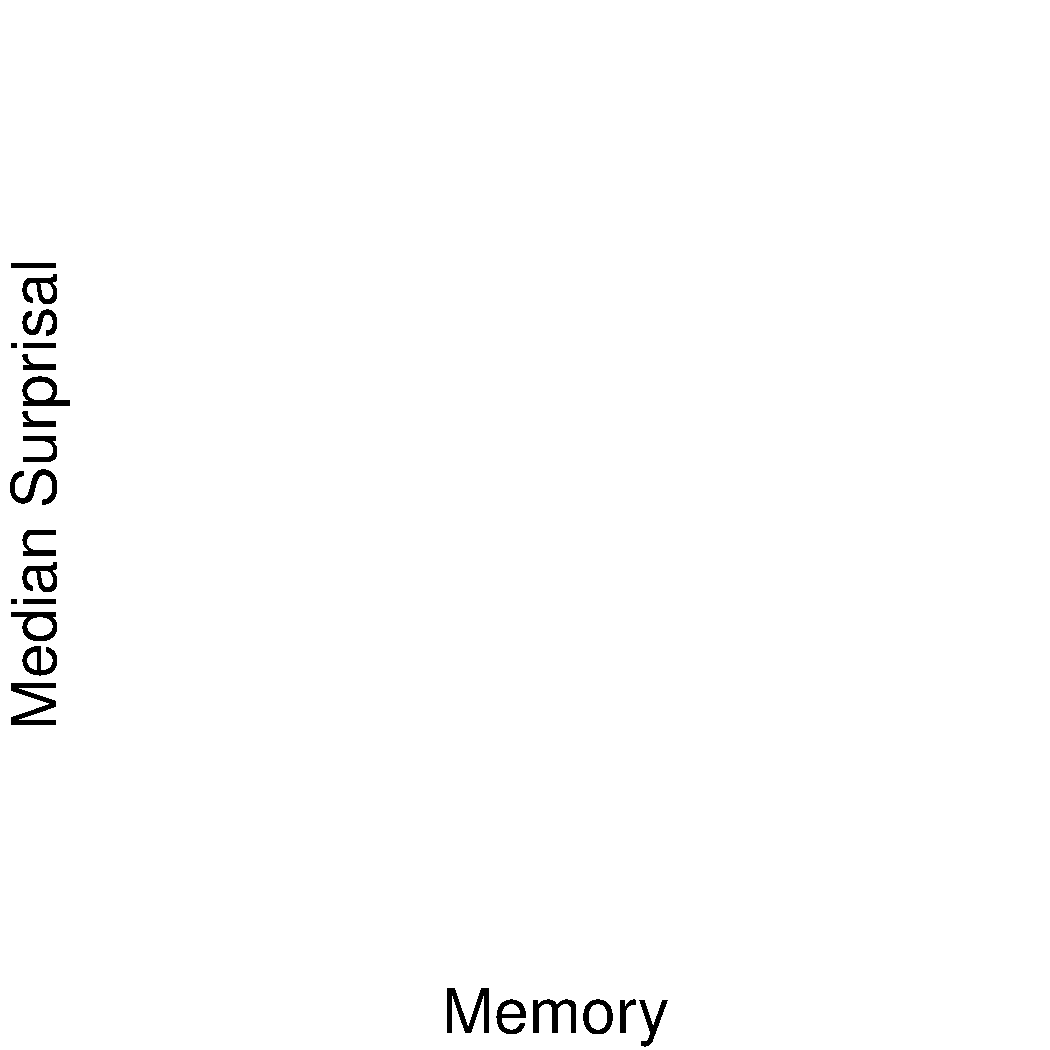
\includegraphics[width=0.25\textwidth]{../code/analyze_ngrams/visualize/figures/Slovenian-listener-surprisal-memory-MEDIANS_onlyWordForms_boundedVocab.pdf} & 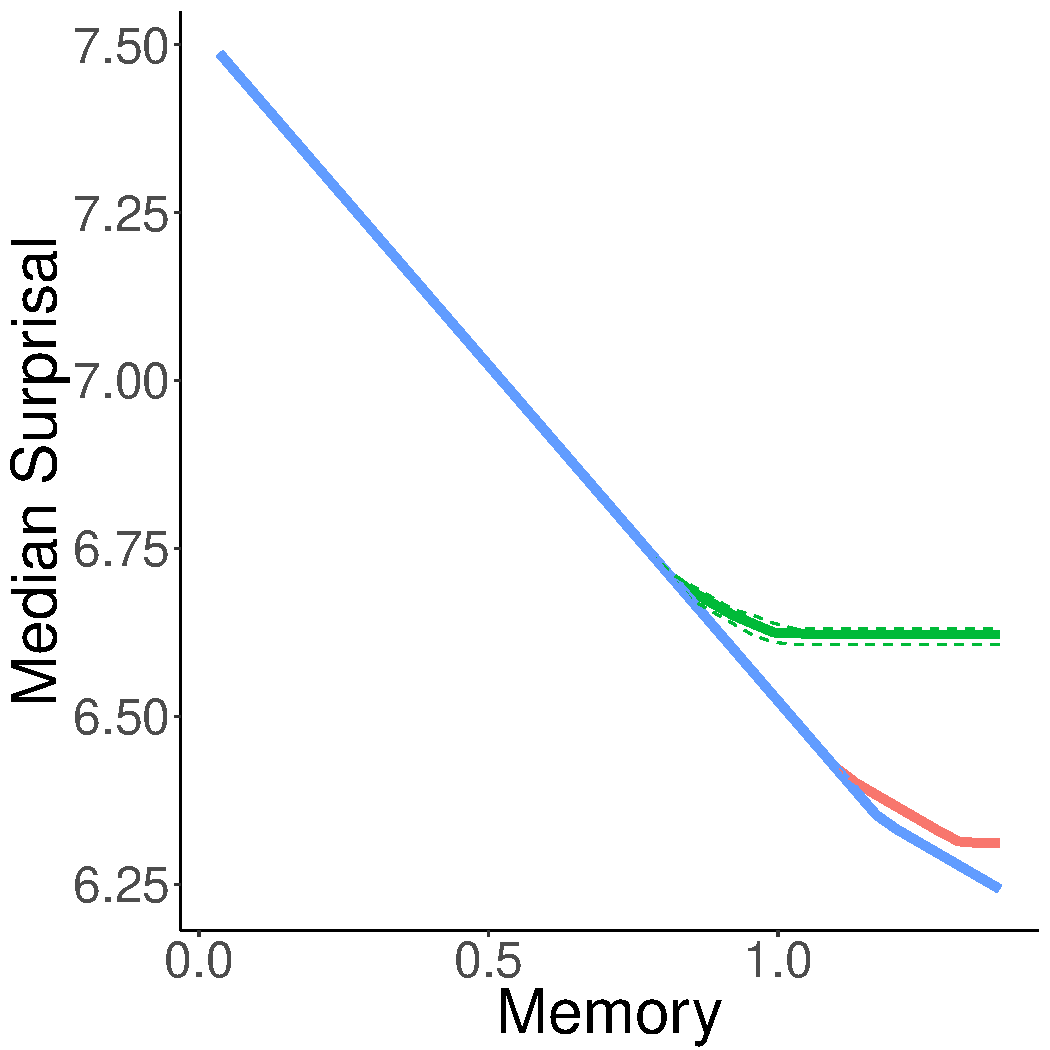
\includegraphics[width=0.25\textwidth]{../code/analyze_ngrams/visualize/figures/Spanish-listener-surprisal-memory-MEDIANS_onlyWordForms_boundedVocab.pdf} & 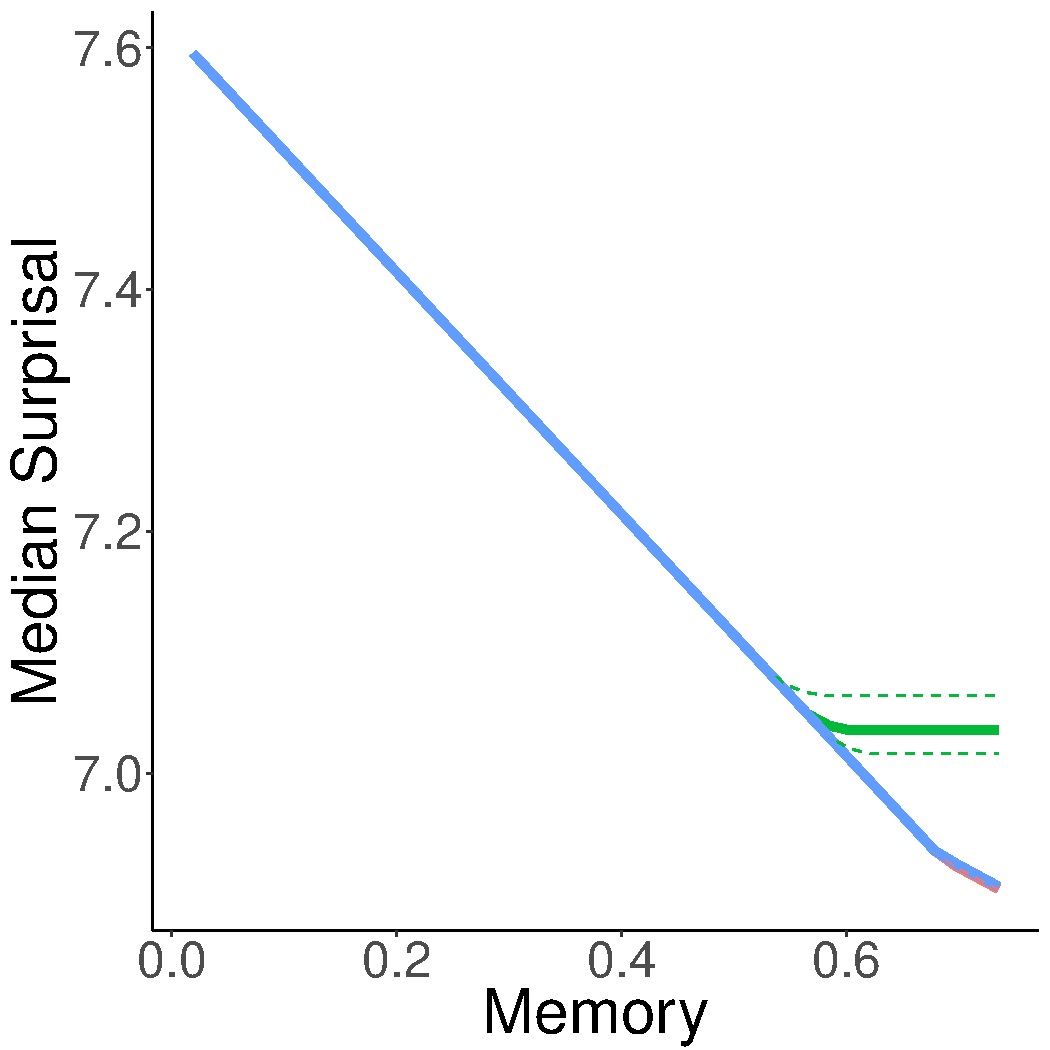
\includegraphics[width=0.25\textwidth]{../code/analyze_ngrams/visualize/figures/Swedish-listener-surprisal-memory-MEDIANS_onlyWordForms_boundedVocab.pdf}
 \\ 

Thai & Turkish & Ukrainian & Urdu
 \\ 
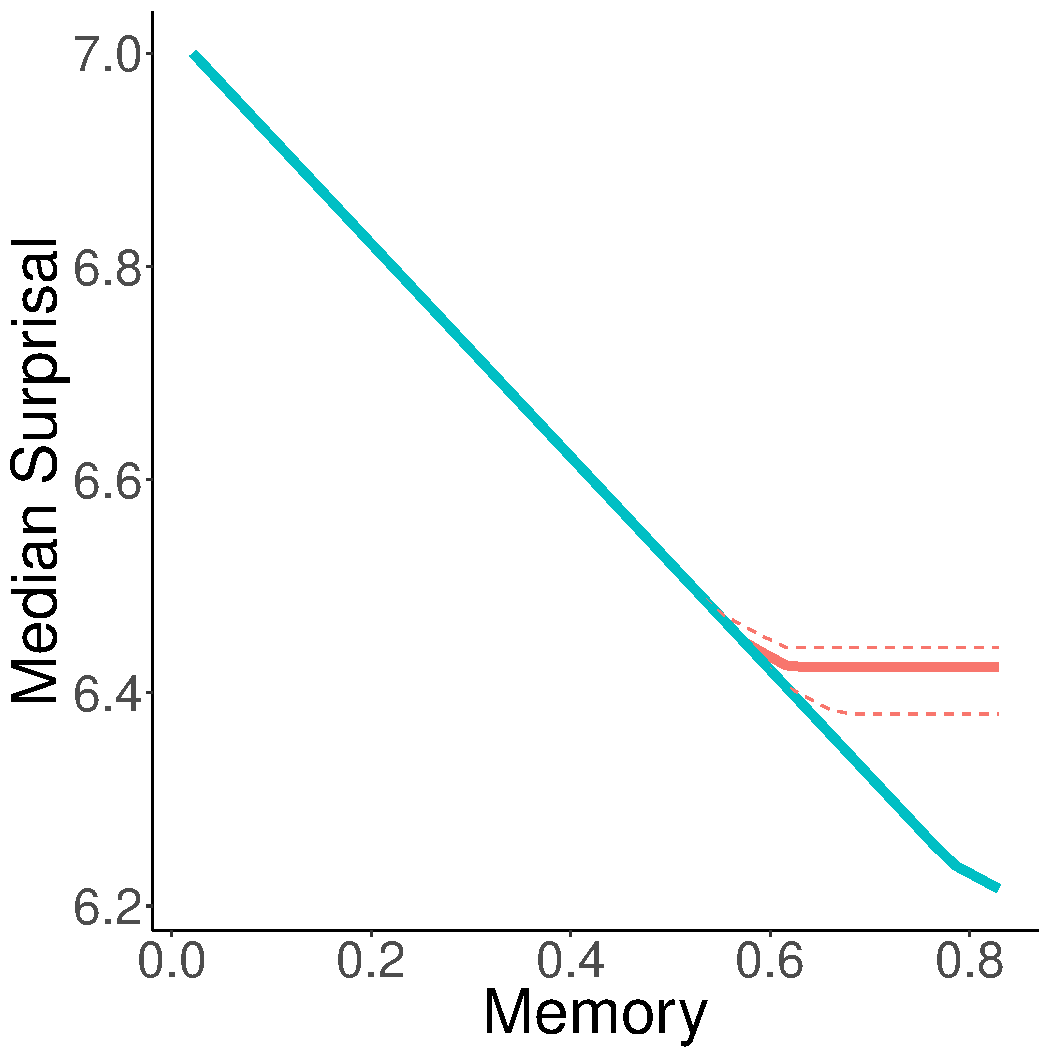
\includegraphics[width=0.25\textwidth]{../code/analyze_ngrams/visualize/figures/Thai-Adap-listener-surprisal-memory-MEDIANS_onlyWordForms_boundedVocab.pdf} & 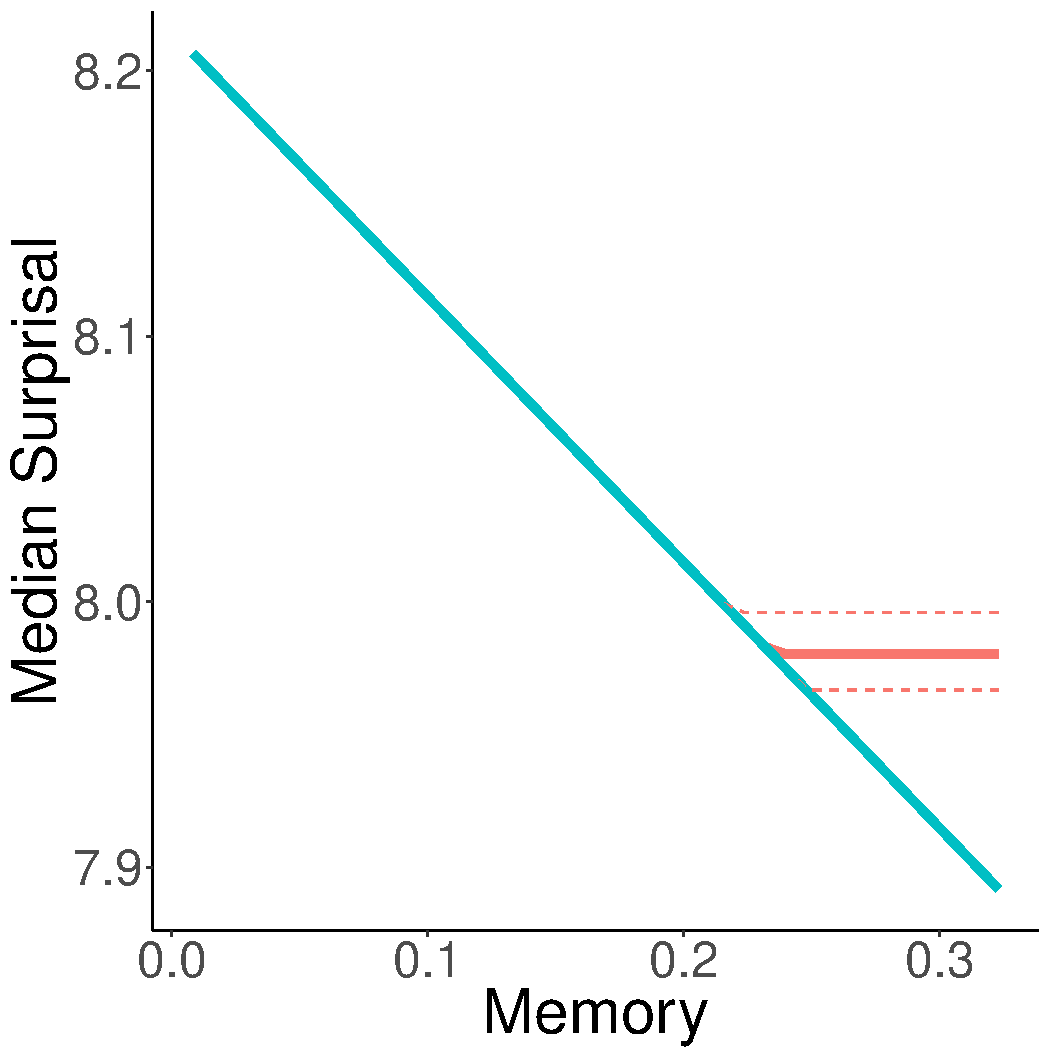
\includegraphics[width=0.25\textwidth]{../code/analyze_ngrams/visualize/figures/Turkish-listener-surprisal-memory-MEDIANS_onlyWordForms_boundedVocab.pdf} & 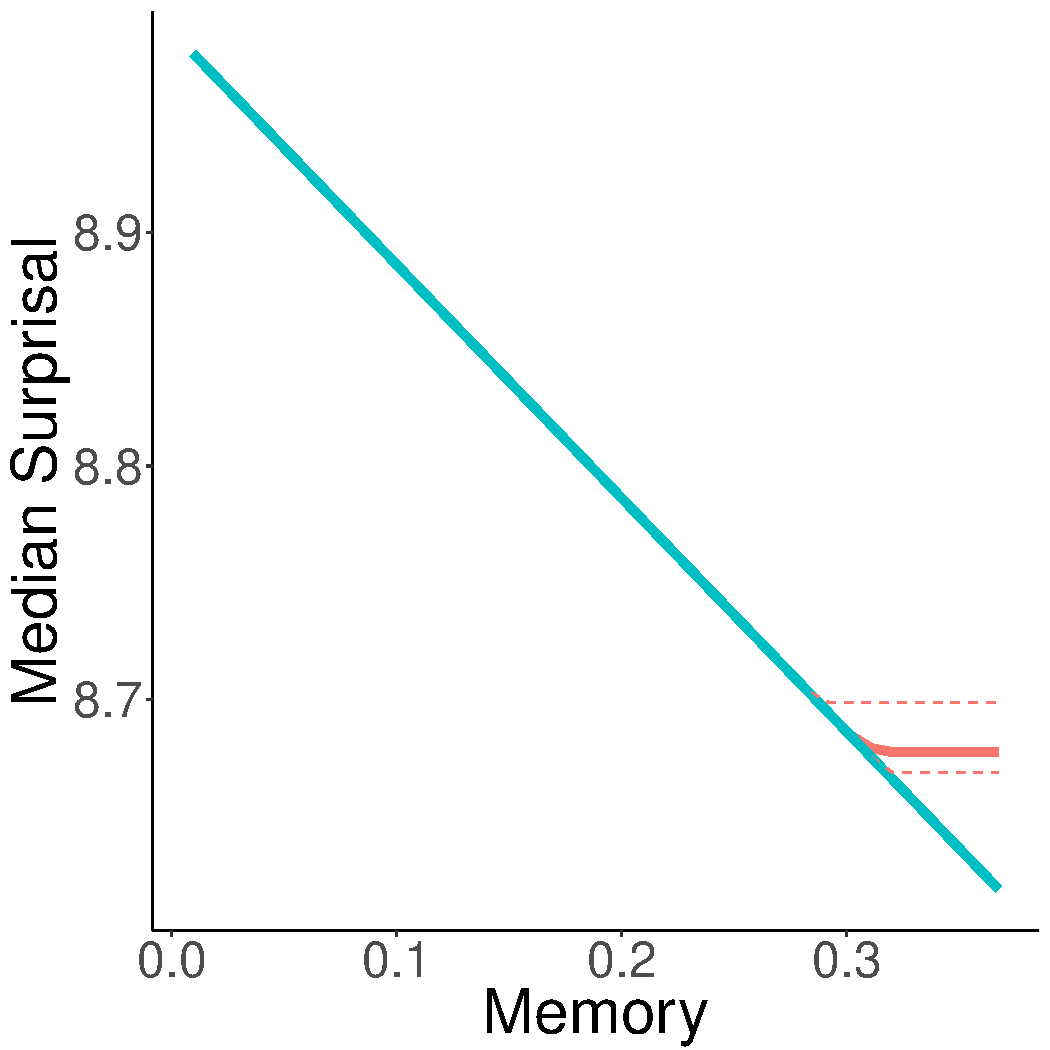
\includegraphics[width=0.25\textwidth]{../code/analyze_ngrams/visualize/figures/Ukrainian-listener-surprisal-memory-MEDIANS_onlyWordForms_boundedVocab.pdf} & 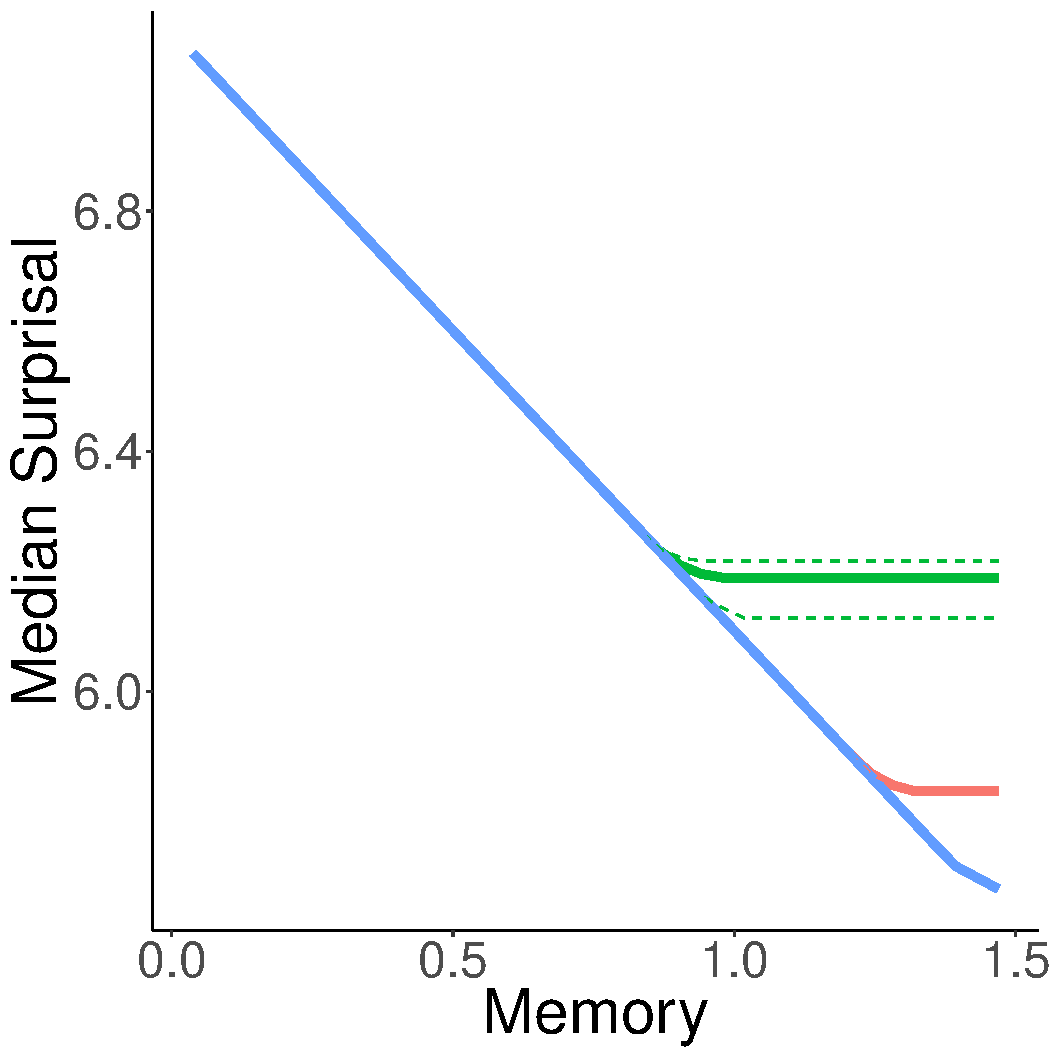
\includegraphics[width=0.25\textwidth]{../code/analyze_ngrams/visualize/figures/Urdu-listener-surprisal-memory-MEDIANS_onlyWordForms_boundedVocab.pdf}
 \\ 
Uyghur & Vietnamese &  & 
 \\ 
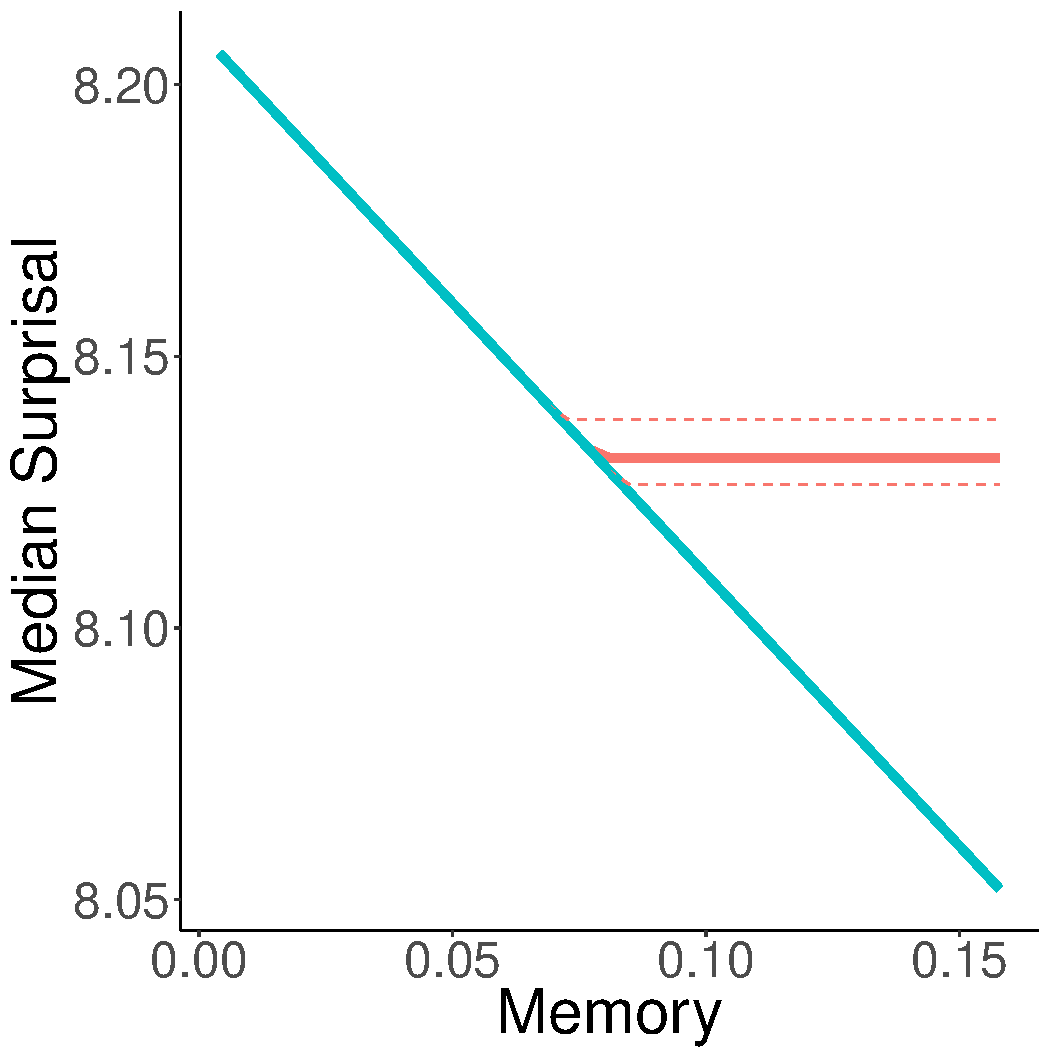
\includegraphics[width=0.25\textwidth]{../code/analyze_ngrams/visualize/figures/Uyghur-Adap-listener-surprisal-memory-MEDIANS_onlyWordForms_boundedVocab.pdf} & 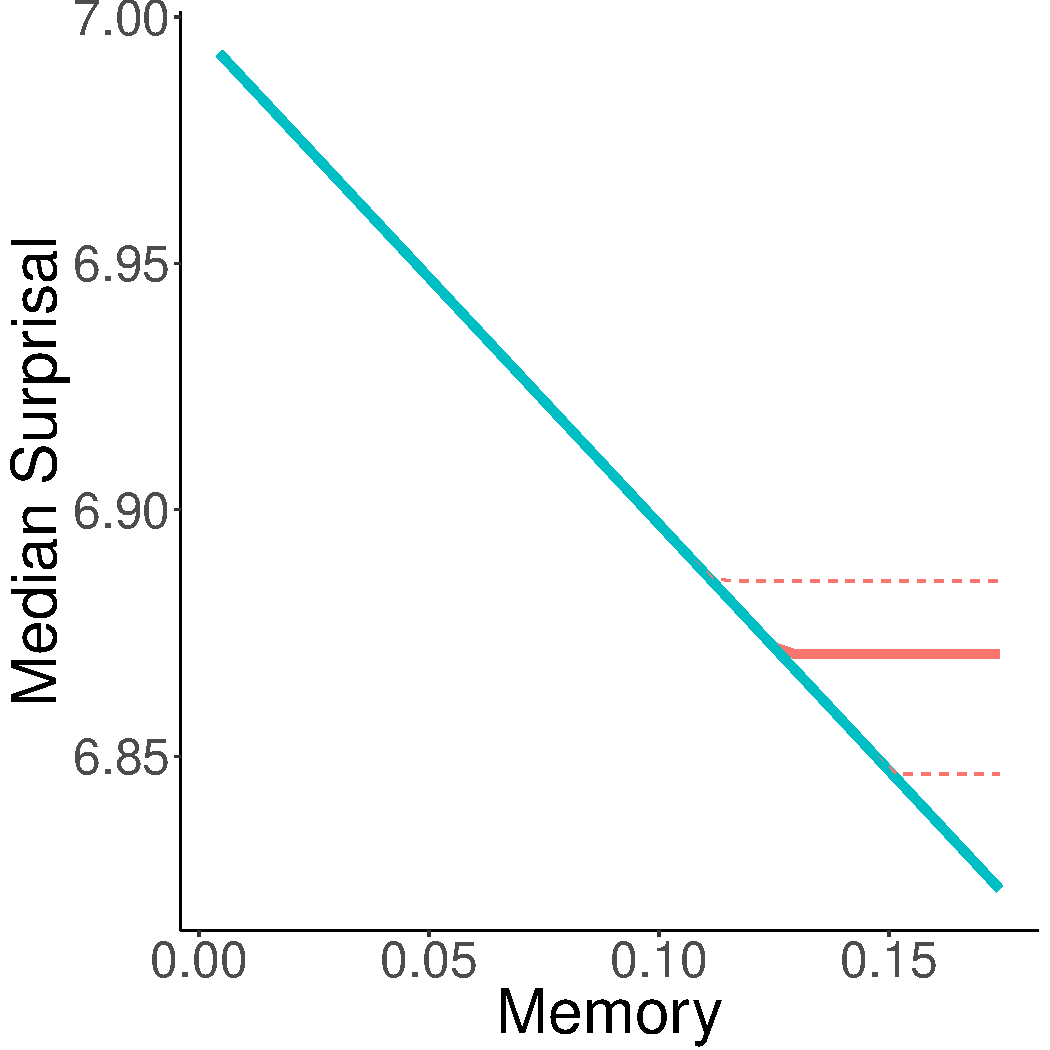
\includegraphics[width=0.25\textwidth]{../code/analyze_ngrams/visualize/figures/Vietnamese-listener-surprisal-memory-MEDIANS_onlyWordForms_boundedVocab.pdf} &  & 
 \\ 

\end{longtable}
	\captionof{figure}{Medians (estimated using n-gram models): For each memory budget, we provide the median surprisal for real and random languages. Solid lines indicate sample medians for ngrams, dashed lines indicate 95 \% confidence intervals for the population median. Green: Random baselines; blue: real language; red: maximum-likelihood grammars fit to real orderings.}\label{tab:medians_ngrams}
\end{center}




% ../../writeup/tables/quantiles_REAL_NGRAMS_0.tex
%
%\begin{center}
%\begin{longtable}{cccccccccccccccccc}
%Afrikaans & Amharic & Arabic & Armenian
 \\ 
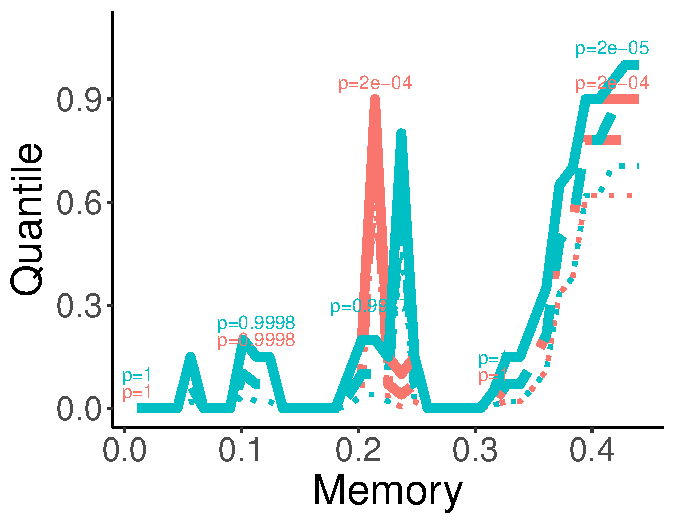
\includegraphics[width=0.25\textwidth]{ngrams/figures/Afrikaans-listener-surprisal-memory-QUANTILES_onlyWordForms_boundedVocab_REAL_NGRAMS.pdf} & 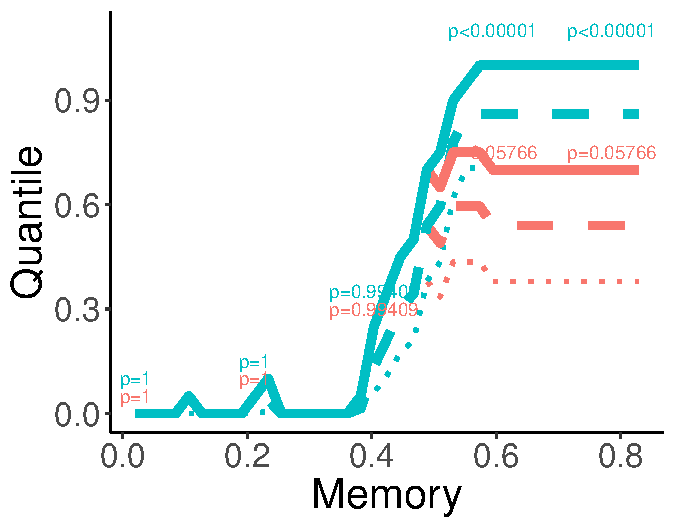
\includegraphics[width=0.25\textwidth]{ngrams/figures/Amharic-Adap-listener-surprisal-memory-QUANTILES_onlyWordForms_boundedVocab_REAL_NGRAMS.pdf} & \includegraphics[width=0.25\textwidth]{ngrams/figures/Arabic-listener-surprisal-memory-QUANTILES_onlyWordForms_boundedVocab_REAL_NGRAMS.pdf} & \includegraphics[width=0.25\textwidth]{ngrams/figures/Armenian-Adap-listener-surprisal-memory-QUANTILES_onlyWordForms_boundedVocab_REAL_NGRAMS.pdf}
 \\ 
Bambara & Basque & Breton & Bulgarian
 \\ 
\includegraphics[width=0.25\textwidth]{ngrams/figures/Bambara-Adap-listener-surprisal-memory-QUANTILES_onlyWordForms_boundedVocab_REAL_NGRAMS.pdf} & \includegraphics[width=0.25\textwidth]{ngrams/figures/Basque-listener-surprisal-memory-QUANTILES_onlyWordForms_boundedVocab_REAL_NGRAMS.pdf} & \includegraphics[width=0.25\textwidth]{ngrams/figures/Breton-Adap-listener-surprisal-memory-QUANTILES_onlyWordForms_boundedVocab_REAL_NGRAMS.pdf} & \includegraphics[width=0.25\textwidth]{ngrams/figures/Bulgarian-listener-surprisal-memory-QUANTILES_onlyWordForms_boundedVocab_REAL_NGRAMS.pdf}
 \\ 
Buryat & Cantonese & Catalan & Chinese
 \\ 
\includegraphics[width=0.25\textwidth]{ngrams/figures/Buryat-Adap-listener-surprisal-memory-QUANTILES_onlyWordForms_boundedVocab_REAL_NGRAMS.pdf} & \includegraphics[width=0.25\textwidth]{ngrams/figures/Cantonese-Adap-listener-surprisal-memory-QUANTILES_onlyWordForms_boundedVocab_REAL_NGRAMS.pdf} & \includegraphics[width=0.25\textwidth]{ngrams/figures/Catalan-listener-surprisal-memory-QUANTILES_onlyWordForms_boundedVocab_REAL_NGRAMS.pdf} & \includegraphics[width=0.25\textwidth]{ngrams/figures/Chinese-listener-surprisal-memory-QUANTILES_onlyWordForms_boundedVocab_REAL_NGRAMS.pdf}
 \\ 
Croatian & Czech & Danish & Dutch
 \\ 
\includegraphics[width=0.25\textwidth]{ngrams/figures/Croatian-listener-surprisal-memory-QUANTILES_onlyWordForms_boundedVocab_REAL_NGRAMS.pdf} & \includegraphics[width=0.25\textwidth]{ngrams/figures/Czech-listener-surprisal-memory-QUANTILES_onlyWordForms_boundedVocab_REAL_NGRAMS.pdf} & \includegraphics[width=0.25\textwidth]{ngrams/figures/Danish-listener-surprisal-memory-QUANTILES_onlyWordForms_boundedVocab_REAL_NGRAMS.pdf} & \includegraphics[width=0.25\textwidth]{ngrams/figures/Dutch-listener-surprisal-memory-QUANTILES_onlyWordForms_boundedVocab_REAL_NGRAMS.pdf}
 \\ 
English & Erzya & Estonian & Faroese
 \\ 
\includegraphics[width=0.25\textwidth]{ngrams/figures/English-listener-surprisal-memory-QUANTILES_onlyWordForms_boundedVocab_REAL_NGRAMS.pdf} & \includegraphics[width=0.25\textwidth]{ngrams/figures/Erzya-Adap-listener-surprisal-memory-QUANTILES_onlyWordForms_boundedVocab_REAL_NGRAMS.pdf} & \includegraphics[width=0.25\textwidth]{ngrams/figures/Estonian-listener-surprisal-memory-QUANTILES_onlyWordForms_boundedVocab_REAL_NGRAMS.pdf} & \includegraphics[width=0.25\textwidth]{ngrams/figures/Faroese-Adap-listener-surprisal-memory-QUANTILES_onlyWordForms_boundedVocab_REAL_NGRAMS.pdf}
 \\ 

%Finnish & French & German & Greek
 \\ 
\includegraphics[width=0.25\textwidth]{ngrams/figures/Finnish-listener-surprisal-memory-QUANTILES_onlyWordForms_boundedVocab_REAL_NGRAMS.pdf} & \includegraphics[width=0.25\textwidth]{ngrams/figures/French-listener-surprisal-memory-QUANTILES_onlyWordForms_boundedVocab_REAL_NGRAMS.pdf} & \includegraphics[width=0.25\textwidth]{ngrams/figures/German-listener-surprisal-memory-QUANTILES_onlyWordForms_boundedVocab_REAL_NGRAMS.pdf} & \includegraphics[width=0.25\textwidth]{ngrams/figures/Greek-listener-surprisal-memory-QUANTILES_onlyWordForms_boundedVocab_REAL_NGRAMS.pdf}
 \\ 
Hebrew & Hindi & Hungarian & Indonesian
 \\ 
\includegraphics[width=0.25\textwidth]{ngrams/figures/Hebrew-listener-surprisal-memory-QUANTILES_onlyWordForms_boundedVocab_REAL_NGRAMS.pdf} & \includegraphics[width=0.25\textwidth]{ngrams/figures/Hindi-listener-surprisal-memory-QUANTILES_onlyWordForms_boundedVocab_REAL_NGRAMS.pdf} & \includegraphics[width=0.25\textwidth]{ngrams/figures/Hungarian-listener-surprisal-memory-QUANTILES_onlyWordForms_boundedVocab_REAL_NGRAMS.pdf} & \includegraphics[width=0.25\textwidth]{ngrams/figures/Indonesian-listener-surprisal-memory-QUANTILES_onlyWordForms_boundedVocab_REAL_NGRAMS.pdf}
 \\ 
Italian & Japanese & Kazakh & Korean
 \\ 
\includegraphics[width=0.25\textwidth]{ngrams/figures/Italian-listener-surprisal-memory-QUANTILES_onlyWordForms_boundedVocab_REAL_NGRAMS.pdf} & \includegraphics[width=0.25\textwidth]{ngrams/figures/Japanese-listener-surprisal-memory-QUANTILES_onlyWordForms_boundedVocab_REAL_NGRAMS.pdf} & \includegraphics[width=0.25\textwidth]{ngrams/figures/Kazakh-Adap-listener-surprisal-memory-QUANTILES_onlyWordForms_boundedVocab_REAL_NGRAMS.pdf} & \includegraphics[width=0.25\textwidth]{ngrams/figures/Korean-listener-surprisal-memory-QUANTILES_onlyWordForms_boundedVocab_REAL_NGRAMS.pdf}
 \\ 
Kurmanji & Latvian & Maltese & Naija
 \\ 
\includegraphics[width=0.25\textwidth]{ngrams/figures/Kurmanji-Adap-listener-surprisal-memory-QUANTILES_onlyWordForms_boundedVocab_REAL_NGRAMS.pdf} & \includegraphics[width=0.25\textwidth]{ngrams/figures/Latvian-listener-surprisal-memory-QUANTILES_onlyWordForms_boundedVocab_REAL_NGRAMS.pdf} & \includegraphics[width=0.25\textwidth]{ngrams/figures/Maltese-listener-surprisal-memory-QUANTILES_onlyWordForms_boundedVocab_REAL_NGRAMS.pdf} & \includegraphics[width=0.25\textwidth]{ngrams/figures/Naija-Adap-listener-surprisal-memory-QUANTILES_onlyWordForms_boundedVocab_REAL_NGRAMS.pdf}
 \\ 
North Sami & Norwegian & Persian & Polish
 \\ 
\includegraphics[width=0.25\textwidth]{ngrams/figures/North_Sami-listener-surprisal-memory-QUANTILES_onlyWordForms_boundedVocab_REAL_NGRAMS.pdf} & \includegraphics[width=0.25\textwidth]{ngrams/figures/Norwegian-listener-surprisal-memory-QUANTILES_onlyWordForms_boundedVocab_REAL_NGRAMS.pdf} & \includegraphics[width=0.25\textwidth]{ngrams/figures/Persian-listener-surprisal-memory-QUANTILES_onlyWordForms_boundedVocab_REAL_NGRAMS.pdf} & \includegraphics[width=0.25\textwidth]{ngrams/figures/Polish-listener-surprisal-memory-QUANTILES_onlyWordForms_boundedVocab_REAL_NGRAMS.pdf}
 \\ 

%Portuguese & Romanian & Russian & Serbian
 \\ 
\includegraphics[width=0.25\textwidth]{ngrams/figures/Portuguese-listener-surprisal-memory-QUANTILES_onlyWordForms_boundedVocab_REAL_NGRAMS.pdf} & \includegraphics[width=0.25\textwidth]{ngrams/figures/Romanian-listener-surprisal-memory-QUANTILES_onlyWordForms_boundedVocab_REAL_NGRAMS.pdf} & \includegraphics[width=0.25\textwidth]{ngrams/figures/Russian-listener-surprisal-memory-QUANTILES_onlyWordForms_boundedVocab_REAL_NGRAMS.pdf} & \includegraphics[width=0.25\textwidth]{ngrams/figures/Serbian-listener-surprisal-memory-QUANTILES_onlyWordForms_boundedVocab_REAL_NGRAMS.pdf}
 \\ 
Slovak & Slovenian & Spanish & Swedish
 \\ 
\includegraphics[width=0.25\textwidth]{ngrams/figures/Slovak-listener-surprisal-memory-QUANTILES_onlyWordForms_boundedVocab_REAL_NGRAMS.pdf} & \includegraphics[width=0.25\textwidth]{ngrams/figures/Slovenian-listener-surprisal-memory-QUANTILES_onlyWordForms_boundedVocab_REAL_NGRAMS.pdf} & \includegraphics[width=0.25\textwidth]{ngrams/figures/Spanish-listener-surprisal-memory-QUANTILES_onlyWordForms_boundedVocab_REAL_NGRAMS.pdf} & \includegraphics[width=0.25\textwidth]{ngrams/figures/Swedish-listener-surprisal-memory-QUANTILES_onlyWordForms_boundedVocab_REAL_NGRAMS.pdf}
 \\ 
Thai & Turkish & Ukrainian & Urdu
 \\ 
\includegraphics[width=0.25\textwidth]{ngrams/figures/Thai-Adap-listener-surprisal-memory-QUANTILES_onlyWordForms_boundedVocab_REAL_NGRAMS.pdf} & \includegraphics[width=0.25\textwidth]{ngrams/figures/Turkish-listener-surprisal-memory-QUANTILES_onlyWordForms_boundedVocab_REAL_NGRAMS.pdf} & \includegraphics[width=0.25\textwidth]{ngrams/figures/Ukrainian-listener-surprisal-memory-QUANTILES_onlyWordForms_boundedVocab_REAL_NGRAMS.pdf} & \includegraphics[width=0.25\textwidth]{ngrams/figures/Urdu-listener-surprisal-memory-QUANTILES_onlyWordForms_boundedVocab_REAL_NGRAMS.pdf}
 \\ 
Uyghur & Vietnamese &  & 
 \\ 
\includegraphics[width=0.25\textwidth]{ngrams/figures/Uyghur-Adap-listener-surprisal-memory-QUANTILES_onlyWordForms_boundedVocab_REAL_NGRAMS.pdf} & \includegraphics[width=0.25\textwidth]{ngrams/figures/Vietnamese-listener-surprisal-memory-QUANTILES_onlyWordForms_boundedVocab_REAL_NGRAMS.pdf} &  & 
 \\ 

%\end{longtable}
%	\captionof{figure}{Quantiles: At a given memory budget, what percentage of the baselines results in higher listener surprisal than the real language? Solid curves represent sample means, dashed lines represent 95 \% confidence bounds; dotted lines represent 99.9 \% confidence bounds. At five evenly spaced memory levels, we provide a p-value for the null hypothesis that the actual population mean is $0.5$ or less. Confidence bounds and p-values are obtained using an exact nonparametric method (see text).}\label{tab:quantiles}
%\end{center}
%
%bounds.append(["alpha", float, 0.95, 1.0]) # + [x/20.0 for x in range(15, 21)])
%bounds.append(["gamma", int, 1, 2, 3, 4, 5, 8, 10, 15, 20, 25, 30]) # , 200, 300
%bounds.append(["delta", int, 0.1, 0.2, 0.5, 1.0 , 2.0, 3.0, 4.0, 5.0, 8.0, 10.0]) #, 1024]) #, 1024]) # 64, 128,
%bounds.append(["cutoff", int, 2,3,4,5,6,7,8,9,10]) #,7,8,9,10]) #, 1024]) #, 1024]) # 64, 128,
%

